\PassOptionsToPackage{unicode=true}{hyperref} % options for packages loaded elsewhere
\PassOptionsToPackage{hyphens}{url}
\PassOptionsToPackage{dvipsnames,svgnames*,x11names*}{xcolor}
%
\documentclass[brazil,a4paper,oneside,openright,parskip=full]{book}

%------------------------------for url-sensitive linebreaks (needed by XeLaTex)

%--------------------------------------for fitch-style natural deduction proofs

%--------------------for advanced math typesetting (loads all default math pkg)
%----------------------------------------mathematical tools to use with amsmath
  \usepackage{mathtools}
%-----------------------------------------ams mathematical facilities for LaTeX
  %\usepackage{amsmath%----------------possibly loaded loaded somewhere else too
%------------------------------TeX fonts from the american mathematical society
  \usepackage{amsfonts}
%-----------------------------------------------additional mathematical symbols
  %\usepackage{amssymb}%---------------possibly loaded loaded somewhere else too
%---------------------------------typesetting of custom theorems (in ams style)
  \usepackage{amsthm}
%-----------------------------------------------dirac bra-ket and set notations
  \usepackage{braket}
%------------------------for unicode (utf8) math typesettings support for XeTeX
%-------------------------------------for numbered cases (mappings) environment
  \usepackage{cases}
%--------------------------for proof trees in the style of the sequent calculus
  \usepackage{bussproofs}


%--------------------------------to create tabular cells spanning multiple rows

%--to create (tabular cells spanning) multiple columns (load before pkg "bidi")
  \usepackage{multicol}

%------------------------to create continuation headings and legends for floats

%---------to scale graphics relative to reference object (needs pkg "graphicx")
%---------------------usage: \scalerel*{\includegraphics{inlinegraphic.pdf}}{O}
  \usepackage{scalerel}

%----------to not interpret latex commands but display them (see pkg "upquote")

%--------------------------------float (load pkg "float" before pkg "hyperref")

\usepackage{lmodern}
\usepackage{setspace}
\setstretch{1.25}
\usepackage{amssymb,amsmath}
\usepackage{ifxetex,ifluatex}
\usepackage{fixltx2e} % provides \textsubscript
\usepackage{dirtree}
\ifnum 0\ifxetex 1\fi\ifluatex 1\fi=0 % if pdftex
  \usepackage[T1]{fontenc}
  \usepackage[utf8]{inputenc}
  \usepackage{textcomp} % provides euro and other symbols
\else % if luatex or xelatex
  \usepackage{unicode-math}
  \defaultfontfeatures{Ligatures=TeX,Scale=MatchLowercase}
\fi
% use upquote if available, for straight quotes in verbatim environments
\IfFileExists{upquote.sty}{\usepackage{upquote}}{}
% use microtype if available
\IfFileExists{microtype.sty}{%
\usepackage[final]{microtype}
\UseMicrotypeSet[protrusion]{basicmath} % disable protrusion for tt fonts
}{}
\IfFileExists{parskip.sty}{%
\usepackage{parskip}
}{% else
\setlength{\parindent}{0pt}
\setlength{\parskip}{6pt plus 2pt minus 1pt}
}
\usepackage{xcolor}
\usepackage{hyperref}
\hypersetup{
            pdftitle={Desenvolvimento web com Django},
            pdfauthor={Jackson Gomes \textbackslash{} jgomes@ceulp.edu.br},
            colorlinks=true,
            linkcolor=Maroon,
            citecolor=Blue,
            urlcolor=Blue,
            breaklinks=true}
\urlstyle{same}  % don't use monospace font for urls
\usepackage[margin=3cm]{geometry}
%-----------------------listings to typeset source code (see pkg "listings-ex")
\usepackage{listings}
\newcommand{\passthrough}[1]{#1}
\renewcommand{\lstlistingname}{Código-fonte}% Listing -> Algorithm
\renewcommand{\lstlistlistingname}{Lista de Códigos-fontes}% List of Listings -> List of Algorithms
%
% listing colors
%
\definecolor{listing-background}{HTML}{F7F7F7}
\definecolor{listing-rule}{HTML}{B3B2B3}
\definecolor{listing-numbers}{HTML}{B3B2B3}
\definecolor{listing-text-color}{HTML}{000000}
\definecolor{listing-keyword}{HTML}{435489}
\definecolor{listing-identifier}{HTML}{435489}
\definecolor{listing-string}{HTML}{00999A}
\definecolor{listing-comment}{HTML}{8E8E8E}
\definecolor{listing-javadoc-comment}{HTML}{006CA9}
\lstdefinestyle{eisvogel_listing_style}{
  numbers          = left,
  backgroundcolor  = \color{listing-background},
  basicstyle       = \color{listing-text-color}\small\ttfamily{}\linespread{1.15}, % print whole listing small
  xleftmargin      = 2.7em,
  breaklines       = true,
  frame            = bt,
  framesep         = 0.6mm,
  rulecolor        = \color{listing-rule},
  frameround       = ffff,
  framexleftmargin = 2.5em,
  tabsize          = 4,
  numberstyle      = \color{listing-numbers},
  aboveskip        = 2.0em,
  belowcaptionskip = 2.0em,
  keywordstyle     = \color{listing-keyword}\bfseries,
  classoffset      = 0,
  sensitive        = true,
  identifierstyle  = \color{listing-identifier},
  commentstyle     = \color{listing-comment},
  morecomment      = [s][\color{listing-javadoc-comment}]{/**}{*/},
  stringstyle      = \color{listing-string},
  showstringspaces = false,
  escapeinside     = {/*@}{@*/}, % Allow LaTeX inside these special comments
  literate         =
  {á}{{\'a}}1 {é}{{\'e}}1 {í}{{\'i}}1 {ó}{{\'o}}1 {ú}{{\'u}}1
  {Á}{{\'A}}1 {É}{{\'E}}1 {Í}{{\'I}}1 {Ó}{{\'O}}1 {Ú}{{\'U}}1
  {à}{{\`a}}1 {è}{{\'e}}1 {ì}{{\`i}}1 {ò}{{\`o}}1 {ù}{{\`u}}1
  {À}{{\`A}}1 {È}{{\'E}}1 {Ì}{{\`I}}1 {Ò}{{\`O}}1 {Ù}{{\`U}}1
  {ä}{{\"a}}1 {ë}{{\"e}}1 {ï}{{\"i}}1 {ö}{{\"o}}1 {ü}{{\"u}}1
  {Ä}{{\"A}}1 {Ë}{{\"E}}1 {Ï}{{\"I}}1 {Ö}{{\"O}}1 {Ü}{{\"U}}1
  {â}{{\^a}}1 {ê}{{\^e}}1 {î}{{\^i}}1 {ô}{{\^o}}1 {û}{{\^u}}1
  {Â}{{\^A}}1 {Ê}{{\^E}}1 {Î}{{\^I}}1 {Ô}{{\^O}}1 {Û}{{\^U}}1
  {œ}{{\oe}}1 {Œ}{{\OE}}1 {æ}{{\ae}}1 {Æ}{{\AE}}1 {ß}{{\ss}}1
  {ç}{{\c c}}1 {Ç}{{\c C}}1 {ø}{{\o}}1 {å}{{\r a}}1 {Å}{{\r A}}1
  {€}{{\EUR}}1 {£}{{\pounds}}1 {«}{{\guillemotleft}}1
  {»}{{\guillemotright}}1 {ñ}{{\~n}}1 {Ñ}{{\~N}}1 {¿}{{?`}}1
  {…}{{\ldots}}1 {≥}{{>=}}1 {≤}{{<=}}1 {„}{{\glqq}}1 {“}{{\grqq}}1
  {”}{{''}}1
}
\lstdefinestyle{nonumber}{
  numbers          = none,
  backgroundcolor  = \color{listing-background},
  basicstyle       = \color{listing-text-color}\small\ttfamily{}\linespread{1.15}, % print whole listing small
  xleftmargin      = 0em,
  breaklines       = true,
  frame            = bt,
  framesep         = 0.6mm,
  rulecolor        = \color{listing-rule},
  frameround       = ffff,
  framexleftmargin = 0em,
  tabsize          = 4,
  aboveskip        = 2.0em,
  belowcaptionskip = 2.0em,
  keywordstyle     = \color{listing-keyword}\bfseries,
  classoffset      = 0,
  sensitive        = true,
  identifierstyle  = \color{listing-identifier},
  commentstyle     = \color{listing-comment},
  morecomment      = [s][\color{listing-javadoc-comment}]{/**}{*/},
  stringstyle      = \color{listing-string},
  showstringspaces = false,
  escapeinside     = {/*@}{@*/}, % Allow LaTeX inside these special comments
  literate         =
  {á}{{\'a}}1 {é}{{\'e}}1 {í}{{\'i}}1 {ó}{{\'o}}1 {ú}{{\'u}}1
  {Á}{{\'A}}1 {É}{{\'E}}1 {Í}{{\'I}}1 {Ó}{{\'O}}1 {Ú}{{\'U}}1
  {à}{{\`a}}1 {è}{{\'e}}1 {ì}{{\`i}}1 {ò}{{\`o}}1 {ù}{{\`u}}1
  {À}{{\`A}}1 {È}{{\'E}}1 {Ì}{{\`I}}1 {Ò}{{\`O}}1 {Ù}{{\`U}}1
  {ä}{{\"a}}1 {ë}{{\"e}}1 {ï}{{\"i}}1 {ö}{{\"o}}1 {ü}{{\"u}}1
  {Ä}{{\"A}}1 {Ë}{{\"E}}1 {Ï}{{\"I}}1 {Ö}{{\"O}}1 {Ü}{{\"U}}1
  {â}{{\^a}}1 {ê}{{\^e}}1 {î}{{\^i}}1 {ô}{{\^o}}1 {û}{{\^u}}1
  {Â}{{\^A}}1 {Ê}{{\^E}}1 {Î}{{\^I}}1 {Ô}{{\^O}}1 {Û}{{\^U}}1
  {œ}{{\oe}}1 {Œ}{{\OE}}1 {æ}{{\ae}}1 {Æ}{{\AE}}1 {ß}{{\ss}}1
  {ç}{{\c c}}1 {Ç}{{\c C}}1 {ø}{{\o}}1 {å}{{\r a}}1 {Å}{{\r A}}1
  {€}{{\EUR}}1 {£}{{\pounds}}1 {«}{{\guillemotleft}}1
  {»}{{\guillemotright}}1 {ñ}{{\~n}}1 {Ñ}{{\~N}}1 {¿}{{?`}}1
  {…}{{\ldots}}1 {≥}{{>=}}1 {≤}{{<=}}1 {„}{{\glqq}}1 {“}{{\grqq}}1
  {”}{{''}}1
}
\lstset{style=eisvogel_listing_style}

\lstdefinelanguage{XML}{
  morestring      = [b]",
  moredelim       = [s][\bfseries\color{listing-keyword}]{<}{\ },
  moredelim       = [s][\bfseries\color{listing-keyword}]{</}{>},
  moredelim       = [l][\bfseries\color{listing-keyword}]{/>},
  moredelim       = [l][\bfseries\color{listing-keyword}]{>},
  morecomment     = [s]{<?}{?>},
  morecomment     = [s]{<!--}{-->},
  commentstyle    = \color{listing-comment},
  stringstyle     = \color{listing-string},
  identifierstyle = \color{listing-identifier}
}
\usepackage{graphicx,grffile,rotating}
\makeatletter
\def\maxwidth{\ifdim\Gin@nat@width>\linewidth\linewidth\else\Gin@nat@width\fi}
\def\maxheight{\ifdim\Gin@nat@height>\textheight\textheight\else\Gin@nat@height\fi}
\makeatother
% Scale images if necessary, so that they will not overflow the page
% margins by default, and it is still possible to overwrite the defaults
% using explicit options in \includegraphics[width, height, ...]{}
\setkeys{Gin}{width=\maxwidth,height=\maxheight,keepaspectratio}
\setlength{\emergencystretch}{3em}  % prevent overfull lines
\providecommand{\tightlist}{%
  \setlength{\itemsep}{0pt}\setlength{\parskip}{0pt}}
\setcounter{secnumdepth}{3}
% Redefines (sub)paragraphs to behave more like sections
\ifx\paragraph\undefined\else
\let\oldparagraph\paragraph
\renewcommand{\paragraph}[1]{\oldparagraph{#1}\mbox{}}
\fi
\ifx\subparagraph\undefined\else
\let\oldsubparagraph\subparagraph
\renewcommand{\subparagraph}[1]{\oldsubparagraph{#1}\mbox{}}
\fi
\pagestyle{headings}

% set default figure placement to htbp
\makeatletter
\def\fps@figure{htbp}
\makeatother

\makeatletter
\@ifpackageloaded{subfig}{}{\usepackage{subfig}}
\@ifpackageloaded{caption}{}{\usepackage{caption}}
\captionsetup[subfloat]{margin=0.5em}
\AtBeginDocument{%
\renewcommand*\figurename{Figura}
\renewcommand*\tablename{Tabela}
}
\AtBeginDocument{%
\renewcommand*\listfigurename{Lista de Figuras}
\renewcommand*\listtablename{Lista de Tabelas}
}
\newcommand*\listoflistings\lstlistoflistings
\AtBeginDocument{%
\renewcommand*{\lstlistlistingname}{Lista de Códigos-fontes}
}
\makeatother
%--------load polyglossia as late as possible BUT BEFORE bidi as it*could* call
%--------------------------------------------------------------bidi if RTL lang
%-------------------------------------------------------(e.g. Hebrew or Arabic)
%------------------------polyglossia is a babel replacement (needed by XeLaTeX)
  \usepackage{polyglossia}
  \setmainlanguage[]{brazil}
\ifxetex
  % load bidi as late as possible as it modifies e.g. graphicx
    \usepackage{bidi}
  \fi
\ifnum 0\ifxetex 1\fi\ifluatex 1\fi=0 % if pdftex
  \TeXXeTstate=1
  \newcommand{\RL}[1]{\beginR #1\endR}
  \newcommand{\LR}[1]{\beginL #1\endL}
  \newenvironment{RTL}{\beginR}{\endR}
  \newenvironment{LTR}{\beginL}{\endL}
\fi

\title{Desenvolvimento web com Django}
\providecommand{\subtitle}[1]{}
\subtitle{Ferramentas modernas para desenvolvimento de software web}
\author{Jackson Gomes \textbackslash{} jgomes@ceulp.edu.br}
\providecommand{\institute}[1]{}
\institute{Centro Universitário Luterano de Palmas \and Departamento de Computação \and  \and }
\date{}

\begin{document}
\maketitle

\frontmatter

{
\hypersetup{linkcolor=}
\setcounter{tocdepth}{3}
\tableofcontents
}
\listoftables
\listoffigures
\lstlistoflistings

\hypertarget{prefuxe1cio}{%
\chapter{Prefácio}\label{prefuxe1cio}}

Este é um livro sobre tecnologias de desenvolvimento de software para a
web com foco no \textbf{Django}, um \emph{framework} de desenvolvimento
web. Um \emph{framework} representa um modelo, uma forma de resolver um
problema. Em termos de desenvolvimento de software para a web um
framework fornece ferramentas (ie. código) para o desenvolvimento de
aplicações. Geralmente o propósito de um framework é agilizar as
atividades de desenvolvimento de software, inclusive, fornecendo código
pronto (componentes, bibliotecas etc.) para resolver problemas comuns,
como uma interface de cadastro.

O objetivo deste livro é fornecer uma ferramenta para o desenvolvimento
de habilidades de desenvolvimento web com Django, com a expectativa de
que você comece aprendendo o básico (o ``hello world'') e conclua com
habilidades necessárias para o desenvolvimento de software que conecta
com banco de dados ou fornece uma API HTTP REST, por exemplo.

\hypertarget{convenuxe7uxf5es}{%
\section{Convenções}\label{convenuxe7uxf5es}}

Os trechos de código apresentados no livro seguem o seguinte padrão:

\begin{itemize}
\tightlist
\item
  \textbf{comandos}: devem ser executados no prompt; começam com o
  símbolo \passthrough{\lstinline!$!}
\item
  \textbf{códigos-fontes}: trechos de códigos-fontes de arquivos
\end{itemize}

A seguir, um exemplo de comando:

\begin{lstlisting}[language=sh, style=nonumber]
$ mkdir hello-world
\end{lstlisting}

O exemplo indica que o comando \passthrough{\lstinline!mkdir!}, com a
opção \passthrough{\lstinline!hello-world!}, deve ser executado no
prompt para criar uma pasta com o nome
\passthrough{\lstinline!hello-world!}.

A seguir, um exemplo de código-fonte:

\begin{lstlisting}[language=Python]
class Pessoa:
    pass
\end{lstlisting}

O exemplo apresenta o código-fonte da classe
\passthrough{\lstinline!Pessoa!}. Em algumas situações, trechos de
código podem ser omitidos ou serem apresentados de forma incompleta,
usando os símbolos \passthrough{\lstinline!...!} e
\passthrough{\lstinline!#!}, como no exemplo a seguir:

\begin{lstlisting}[language=Python]
class Pessoa:
    def __init__(self, nome):
        self.nome = nome
    
    def salvar(self):
        # executa validação dos dados
        ...
        # salva 
        return ModelManager.save(self)
\end{lstlisting}

\hypertarget{ambiente-de-execuuxe7uxe3o-do-python-e-do-django}{%
\section{Ambiente de execução do Python e do
Django}\label{ambiente-de-execuuxe7uxe3o-do-python-e-do-django}}

Este livro é voltado para a versão \textbf{3.x} do Python e versão
\textbf{2.x} do Django. Seção~\ref{sec:apendice-1} apresenta um rápido
tutorial sobre configuração de um ambiente Python com \textbf{pip} e
\textbf{virtualenv} ou \textbf{pipenv}. Essas ferramentas são
fundamentais para a configuração do ambiente de desenvolvimento.

\textbf{pip} é um gerenciador de pacotes para o Python. Uma vez que você
precise de recursos adicionais, pode instalar pacotes. Por exemplo, o
comando a seguir demonstra como instalar o Django:

\textbf{virtualenv} é uma ferramenta utilizada para gerenciar ambientes
de projeto, isolados entre si e do ambiente global do Python. Com isso,
cada projeto pode ter seus pacotes e versões diferentes.

\textbf{pipenv} reúne as funcionalidades do \textbf{pip} e do
\textbf{virtualenv} e é uma alternativa mais moderna para o
desenvolvimento de software Python.

Este livro não leva em consideração o Sistema Operacional do seu
ambiente de desenvolvimento, mas é importante que você se acostume a
certos detalhes e a certas ferramentas, como o \textbf{prompt} ou
\textbf{prompt de comando}.

Além destas ferramentas também são utilizadas:

\begin{itemize}
\tightlist
\item
  \textbf{Git}
\item
  \textbf{Heroku}
\end{itemize}

O \textbf{Git} é um gerenciador de repositórios com recursos de
versionamento de código. É uma ferramenta essencial para o gerenciamento
de código fonte de qualquer software.

O \textbf{Heroku} é um serviço de \textbf{PaaS} (de
\emph{Platform-as-a-Service}). PaaS é um modelo de negócio fornece um
ambiente de execução conforme uma plataforma de programação, como o
Python, um tecnologia de banco de dados, como MySQL e PostgreSQL e ainda
outros recursos, como cache usando Redis.

\begin{quote}
\textbf{Calma!} Não pira! (In)Felizmente você não vai usar todas as
tecnologias lendo o conteúdo desse livro. Fica para outra oportunidade.
\end{quote}

Para utilizar o Heroku você precisa criar uma conta de usuário. Acesse
\url{https://www.heroku.com/} e crie uma conta de usuário.

Depois que tiver criado e validado sua conta de usuário instale o
\textbf{Heroku CLI}, uma ferramenta de linha de comando (prompt) que
fornece uma interface de texto para criar e gerenciar aplicativos
Heroku. Detalhes da instalação dessa ferramenta não são tratados aqui,
mas comece acessando
\url{https://devcenter.heroku.com/articles/heroku-cli}.

\hypertarget{servidor-web}{%
\section{Servidor web}\label{servidor-web}}

Um \textbf{servidor web} é um programa que fornece um serviço de rede
que funciona recebendo e atendendo requisições de clientes. Um
\textbf{cliente}, por exemplo, é o browser.

Um \textbf{cliente} solicita um arquivo ao \textbf{servidor web}, que
recebe a solicitação, atende a solicitação e retorna uma resposta para o
cliente.

Esse modelo é chamado \textbf{cliente-servidor} e, na web, utiliza o
protocolo \textbf{HTTP} (de \emph{Hypertext Transfer Protocol}). O
protocolo HTTP determina as regras da comunicação no modelo
cliente-servidor:

\begin{itemize}
\tightlist
\item
  como o cliente deve enviar uma solicitação para o servidor
\item
  como o servidor deve interpretar a solicitação
\item
  como o servidor deve enviar uma resposta para o cliente
\item
  como o cliente deve interpretar a resposta do servidor
\end{itemize}

Para ilustrar esse processo a Figura~\ref{fig:com-cliente-servidor}
demonstra a comunicação entre cliente e servidor.

\begin{figure}
\hypertarget{fig:com-cliente-servidor}{%
\centering
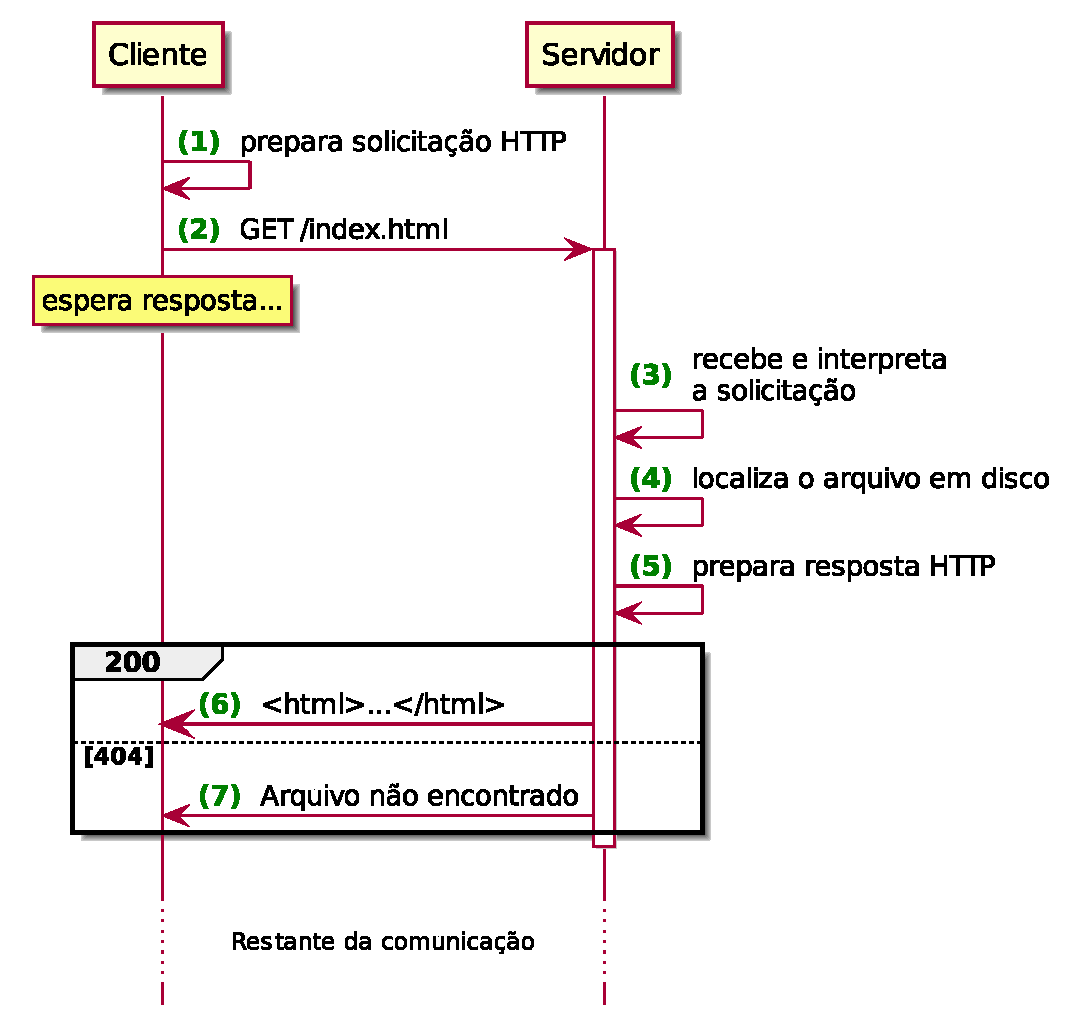
\includegraphics[width=10cm,height=\textheight]{db50a4295b9805759468deef4bdfb3010078ccac.eps}
\caption{Exemplo de comunicação
cliente-servidor\label{fig:com-cliente-servidor}}\label{fig:com-cliente-servidor}
}
\end{figure}

Como a Figura~\ref{fig:com-cliente-servidor} apresenta, quem inicia a
comunicação é o cliente. O servidor recebe a solicitação e retorna uma
resposta. A resposta pode ser interpretada como sucesso ou erro. No caso
da figura, se o servidor encontrar o arquivo, ele retorna um código de
resposta do HTTP com o número 200 e o conteúdo HTML do arquivo
\passthrough{\lstinline!index.html!}, caso contrário ele retorna um
código de resposta HTTP com o número 404, indicando que o arquivo não
foi encontrado.

Como o Django é um framework para desenvolvimento de software esse
processo será bastante utilizado e ficará bastante evidente durante seu
aprendizado.

\mainmatter

\hypertarget{sec:introducao}{%
\chapter{Introdução}\label{sec:introducao}}

O Django surgiu como uma ferramenta para agilizar o desenvolvimento de
software web que, geralmente, tem algumas tarefas comuns. Por exemplo,
um software web tem uma interface administrativa, que permite cadastro e
gerenciamento de dados, e uma interface pública, que permite consulta
dos dados. O Django fornece mecanismos para tornar isso algo bastante
rápido de construir.

A estrutura do Django é baseada no padrão de projeto
\textbf{Model-View-Controller} (MVC). O MVC é um padrão de projeto
arquitetural, o que significa que ele determina, inclusive, como os
elementos do software comunicam entre si. Desta forma:

\begin{itemize}
\tightlist
\item
  \textbf{Model}: representa a camada de dados
\item
  \textbf{View}: representa a interface
\item
  \textbf{Controller}: representa a lógica que liga os dois elementos
  anteriores
\end{itemize}

Falando em \textbf{projeto}, esta é uma unidade importante do Django,
que organiza o software em \textbf{projeto} e seus \textbf{aplicativos}.
Tanto o projeto como o aplicativo são pacotes Python que podem ser
desenvolvidos com o intuito de serem redistribuídos e reutilizados em
outros softwares. Isso ficará mais claro nos capítulos seguintes.

\hypertarget{ambiente-do-projeto-e-dependuxeancias}{%
\section{Ambiente do projeto e
dependências}\label{ambiente-do-projeto-e-dependuxeancias}}

Uma etapa importante de todo projeto Django é a configuração do
ambiente. Antes de prosseguir, garanta que seu ambiente esteja com as
ferramentas devidamente configuradas. Além disso, como há mais de uma
forma de gerenciar pacotes do projeto, o restante desse livro não vai
indicar qual ferramenta utilizar, mas considerar que você já sabe
realizar essa tarefa.

O \textbf{Django} é distribuído como um pacote do Python. Isso significa
que o ambiente do seu projeto precisa ter instalado o pacote
\passthrough{\lstinline!django!}.

A seção a seguir demonstra como criar um \textbf{hello world} Django.

\hypertarget{hello-world-django}{%
\section{Hello World, Django!}\label{hello-world-django}}

Crie uma pasta para seu projeto utilizando o programa
\passthrough{\lstinline!mkdir!} (ou outra forma). Por exemplo, considere
que a pasta do projeto se chame
\passthrough{\lstinline!hello-world-django!}. Em seguida, acesse a pasta
utilizando o programa \passthrough{\lstinline!cd!}.

\begin{lstlisting}[language=sh, style=nonumber]
$ mkdir hello-world-django
$ cd hello-world-django
\end{lstlisting}

Realize a ativação do ambiente do projeto e instale o pacote
\passthrough{\lstinline!django!}.

Com o pacote django instalado no ambiente do projeto é hora de criar um
\textbf{projeto django}. Para isso, utilize o programa
\passthrough{\lstinline!django-admin!}. O exemplo a seguir demonstra
como criar o projeto \passthrough{\lstinline!hello\_world\_django!} na
pasta local:

\begin{lstlisting}[language=sh, style=nonumber]
$ django-admin startproject hello_world_django .
\end{lstlisting}

O programa \passthrough{\lstinline!django-admin!} está sendo executado
utilizando, nesta ordem:

\begin{itemize}
\tightlist
\item
  \passthrough{\lstinline!startproject!}: o comando usado para criar um
  projeto (há outros)
\item
  \passthrough{\lstinline!hello\_world\_django!}: o nome do projeto
  django
\item
  \passthrough{\lstinline!.!}: o local do projeto django
  (\passthrough{\lstinline!.!} representa a pasta local)
\end{itemize}

Um \textbf{projeto django} possui uma estrutura de arquivos bastante
particular, veja:

\dirtree{%
 .1 /.
 .2 Pipfile.
 .2 Pipfile.lock.
 .2 hello\_world\_django/.
 .3 \_\_init\_\_.py.
 .3 settings.py.
 .3 urls.py.
 .3 wsgi.py.
 .2 manage.py.
}

Além dos arquivos do gerenciador de pacotes \textbf{pipenv}
(\passthrough{\lstinline!Pipfile!} e
\passthrough{\lstinline!Pipfile.lock!}) estão:

\begin{itemize}
\tightlist
\item
  \passthrough{\lstinline!manage.py!}: um programa Python utilizado para
  executar determinadas tarefas no projeto django
\item
  \passthrough{\lstinline!hello\_world\_django!}: o diretório que contém
  os arquivos do projeto.
\end{itemize}

Os arquivos do projeto django (no diretório
\passthrough{\lstinline!hello\_world\_django!}):

\begin{itemize}
\tightlist
\item
  \passthrough{\lstinline!\_\_init\_\_.py!}: indica que o conteúdo da
  pasta atual pertence a um pacote Python
\item
  \passthrough{\lstinline!settings.py!}: contém configurações do projeto
  django
\item
  \passthrough{\lstinline!urls.py!}: contém especificações de caminhos,
  URLs e \textbf{rotas} do projeto
\item
  \passthrough{\lstinline!wsgi.py!}: contém a configuração de execução
  do projeto django em um servidor web
\end{itemize}

Agora inicie o servidor web local para utilizar o software, executando:

\begin{lstlisting}[language=sh, style=nonumber]
$ python manage.py runserver
\end{lstlisting}

Neste momento você verá uma saída como a seguinte:

\begin{lstlisting}[style=nonumber]
Performing system checks...

System check identified no issues (0 silenced).

You have 14 unapplied migration(s). Your project may not work properly until you apply the migrations for app(s): admin, auth, contenttypes, sessions.
Run 'python manage.py migrate' to apply them.

July 12, 2018 - 00:30:14
Django version 2.0.7, using settings 'hello_world_django.settings'
Starting development server at http://127.0.0.1:8000/
Quit the server with CONTROL-C.
\end{lstlisting}

Essa é a saída do programa Python \passthrough{\lstinline!manage.py!}
com o argumento \passthrough{\lstinline!runserver!}.

Neste momento, use o browser e navegue até
\passthrough{\lstinline!http://localhost:8000!} ou
\passthrough{\lstinline!http://127.0.0.1:8000!}) e você algo como o que
a Figura~\ref{fig:1-hello-world-inicio-browser}.

\begin{figure}
\hypertarget{fig:1-hello-world-inicio-browser}{%
\centering
\includegraphics{./core/1-hello-world-inicio-browser.png}
\caption{Janela do browser carregando o projeto
django}\label{fig:1-hello-world-inicio-browser}
}
\end{figure}

A Figura~\ref{fig:1-hello-world-inicio-browser} apresenta a ``página
inicial'' do projeto Django em execução. Ela é criada automaticamente
pelo Django para servir como uma verificação rápida de que tudo está
realmente funcionando no seu ambiente de desenvolvimneto.

Voltando ao prompt onde você iniciou o servidor web local, perceba que
começam a aparecer algumas linhas de \textbf{log} à medida que o browser
faz solicitações ao servidor web local, por exemplo:

\begin{lstlisting}[style=nonumber]
[12/Jul/2018 00:32:50] "GET / HTTP/1.1" 200 16348
[12/Jul/2018 00:46:40] "GET / HTTP/1.1" 200 16348
[12/Jul/2018 00:46:40] "GET /static/admin/css/fonts.css HTTP/1.1" 200 423
\end{lstlisting}

Essas linhas são geradas pelo servidor web local para demonstrar que
está ocorrendo alguma atividade, ou seja, está recebendo solicitações de
um cliente (o seu browser).

\hypertarget{hello-world-subiu-uxe0s-nuvens}{%
\section{Hello World subiu às
nuvens!}\label{hello-world-subiu-uxe0s-nuvens}}

Enquanto você está utilizando seu servidor web local somente você
consegue acessar seu software web. Por isso, seu software precisa ir
para a nuvem. Para fazer isso vamos utilizar o \textbf{Heroku}. Antes de
continuar, dois conceitos importantes:

\begin{itemize}
\tightlist
\item
  \textbf{ambiente de desenvolvimento}: corresponde ao seu computador,
  contendo os arquivos e recursos que você utiliza para desenvolver o
  software; o software utiliza o servidor web local e só pode ser
  acessado por você
\item
  \textbf{ambiente de produção}: corresponde ao servidor remoto que você
  utiliza para disponibilizar seu software para outras pessoas (no caso,
  o Heroku)
\end{itemize}

É importante estabelecer uma \textbf{regra de ouro}: \emph{só vai para a
produção o que está 100\% funcionando no ambiente de desenvolvimento}.
Utilizar isso como um princípio garante que o software que as pessoas
vão utilizar esteja realmente funcionando como deveria. Em outros
capítulos você vai aprender a dar essa garantia de uma maneira mais
sistemática. Por enquanto, garanta que o servidor web local não
apresente erros.

\hypertarget{configurauxe7uxe3o-inicial-do-heroku}{%
\subsection{Configuração inicial do
Heroku}\label{configurauxe7uxe3o-inicial-do-heroku}}

O Heroku precisa que você crie o arquivo
\passthrough{\lstinline!Procfile!}, que especifica configurções do
ambiente de execução do Python, com o seguinte conteúdo:

\begin{lstlisting}[style=nonumber]
web: gunicorn hello_world_django.wsgi --log-file -
\end{lstlisting}

Isso indica para o Heroku que ele vai utilizar o servidor web
\textbf{gunicorn} que, diferentemente do servidor web local que você
acabou de utilizar, é voltado para o ambiente de produção.

Instale o pacote \passthrough{\lstinline!gunicorn!} no seu ambiente de
projeto.

Altere o arquivo
\passthrough{\lstinline!hello\_world\_django/settings.py!}, modificando
\passthrough{\lstinline!ALLOWED\_HOSTS!} da seguinte forma:

\begin{lstlisting}[language=Python, style=nonumber]
ALLOWED_HOSTS = ['*']
\end{lstlisting}

Essa configuração permite que seu software possa ser acessado a partir
de outros computadores (hosts).

Os arquivos são enviados ao Heroku por meio do \textbf{Git}, por isso é
necessário executar alguns procedimentos, começando pela inicialização
do \textbf{repositório Git local}. Para isso execute o comando:

\begin{lstlisting}[language=sh, style=nonumber]
$ git init
\end{lstlisting}

Depois configure informações do seu usuário:

\begin{lstlisting}[language=sh, style=nonumber]
$ git config user.email "email@servidor.com"
$ git config user.name "Nome do usuário"
\end{lstlisting}

Substitua \passthrough{\lstinline!email@servidor.com!} pelo e-mail
utilizado na sua conta do Heroku.

Em seguida adicione todos os arquivos do diretório autal em um
\textbf{commit}:

\begin{lstlisting}[language=sh, style=nonumber]
$ git add .
\end{lstlisting}

Depois faça um \textbf{commit}:

\begin{lstlisting}[language=sh, style=nonumber]
$ git commit -m "Commit inicial para produção"
\end{lstlisting}

Crie o aplicativo do Heroku usando o comando a seguir:

\begin{lstlisting}[language=sh, style=nonumber]
$ heroku create
\end{lstlisting}

A saída desse comando é importante e é mais ou menos assim:

\begin{lstlisting}[style=nonumber]
Creating app... done, ⬢ lit-sands-61516
https://lit-sands-61516.herokuapp.com/ | https://git.heroku.com/lit-sands-61516.git
\end{lstlisting}

O nome do aplicativo é criado automaticamente pelo Heroku. Nesse caso é
\textbf{lit-sands-61516}. A saída também informa a URL do aplicativo
(\passthrough{\lstinline!https://lit-sands-61516.herokuapp.com!}) e a
URL do \textbf{repositório Git remoto}
(\passthrough{\lstinline!https://git.heroku.com/lit-sands-61516.git!}).

Em seguida, conecte seu repositório Git local com o repositório remoto:

\begin{lstlisting}[language=sh, style=nonumber]
$ heroku git:remote -a lit-sands-61516
\end{lstlisting}

Isso faz com que o Git seja configurado para enviar arquivos para o
Heroku.

Defina uma variável de ambiente para que o Heroku ignore arquivos
estáticos (como arquivos CSS e JavaScript):

\begin{lstlisting}[language=sh, style=nonumber]
$ heroku config:set DISABLE_COLLECTSTATIC=1
\end{lstlisting}

Envie o conteúdo do commit atual para o Heroku:

\begin{lstlisting}[language=sh, style=nonumber]
$ git push heroku master
\end{lstlisting}

O comando atualiza (sincroniza) o repositório local e o repositório
remoto. A saída desse programa deve ser algo parecido com isso:

\begin{lstlisting}[style=nonumber]
Counting objects: 11, done.
Delta compression using up to 8 threads.
Compressing objects: 100% (10/10), done.
Writing objects: 100% (11/11), 3.40 KiB | 1.13 MiB/s, done.
Total 11 (delta 0), reused 0 (delta 0)
remote: Compressing source files... done.
remote: Building source:
remote:
remote: -----> Python app detected
remote: -----> Installing python-3.6.6
remote: -----> Installing pip
remote: -----> Installing dependencies with Pipenv 2018.5.18…
remote:        Installing dependencies from Pipfile.lock (a8faad)…
remote: -----> Discovering process types
remote:        Procfile declares types -> web
remote:
remote: -----> Compressing...
remote:        Done: 59.3M
remote: -----> Launching...
remote:        Released v5
remote:        https://lit-sands-61516.herokuapp.com/ deployed to Heroku
remote:
remote: Verifying deploy... done.
To https://git.heroku.com/lit-sands-61516.git
 * [new branch]      master -> master
\end{lstlisting}

Pela saída é possível entender que o Heroku identifica o ambiente de
execução do Python, as dependências do aplicativo (nesse caso estão no
arquivo \passthrough{\lstinline!Pipfile.lock!}) e o tipo de processo que
vai ser criado (\passthrough{\lstinline!web!}, utilizando
\passthrough{\lstinline!gunicorn!}). Por fim o Heroku disponibiliza o
aplicativo no ambiente de produção (faz o \textbf{deploy}).

Para concluir inicialize o aplicativo no Heroku utilizando o comando:

\begin{lstlisting}[language=sh, style=nonumber]
$ heroku ps:scale web=1
\end{lstlisting}

A saída do comando deve ser algo como:

\begin{lstlisting}[style=nonumber]
Scaling dynos... done, now running web at 1:Free
\end{lstlisting}

Pronto, agora acesse seu aplicativo no endereço informado pelo Heroku
(nesse caso
\passthrough{\lstinline!https://lit-sands-61516.herokuapp.com/!}).
Perceba que o resultado é o mesmo da execução do seu aplicativo no
ambiente local, como ilustra a
Figura~\ref{fig:2-hello-world-remoto-browser}.

\begin{figure}
\hypertarget{fig:2-hello-world-remoto-browser}{%
\centering
\includegraphics{./core/2-hello-world-remoto-browser.png}
\caption{Janela do browser carregando o projeto django no ambiente
remoto (produção)}\label{fig:2-hello-world-remoto-browser}
}
\end{figure}

Para verificar como seu aplicativo está configurado no Heroku, acesse
sua \emph{dashboard}, clique no aplicativo desejado e veja a área de
configuração. A tela inicial (\emph{Overview}) é semelhante ao que
ilustra a Figura~\ref{fig:3-heroku-app-overview}.

\begin{figure}
\hypertarget{fig:3-heroku-app-overview}{%
\centering
\includegraphics{./core/3-heroku-app-overview.png}
\caption{Tela da visão geral do aplicativo no
Heroku}\label{fig:3-heroku-app-overview}
}
\end{figure}

A Figura~\ref{fig:3-heroku-app-overview} ilustra que a tela
\emph{Overview} apresenta os \emph{Add-ons} instalados e permite acessar
a configuração deles, mostra as informações dos \emph{Dynos} (no caso,
utilizando o nível \emph{free}), as últimas atividades e dá acesso a
outras configurações do aplicativo, como \emph{Deploy}.

\hypertarget{conclusuxe3o}{%
\section{Conclusão}\label{conclusuxe3o}}

Esse capítulo apresentou informações sobre o Django, o Heroku e como
funciona o \emph{workflow} (fluxo de trabalho) para utilizar o
\textbf{Git} e o \textbf{Heroku CLI} para manter os repositórios local e
remoto, bem como fazer o \emph{deploy} da aplicação.

A Figura~\ref{fig:workflow-inicio} apresenta um resumo do
\emph{workflow} até aqui.

\begin{figure}
\hypertarget{fig:workflow-inicio}{%
\centering
\includegraphics{4d693cb34d6665010e6167856930010588acd836.eps}
\caption{Workflow para o desenvolvimento com Django e
Heroku\label{fig:workflow-inicio}}\label{fig:workflow-inicio}
}
\end{figure}

Como ilustra a Figura~\ref{fig:workflow-inicio} o processo é baseado na
utilização de uma ferramenta para gerenciando do ambiente do projeto e
suas dependências (\textbf{virtualenv} ou \textbf{pipenv}), \textbf{Git}
e \textbf{Heroku}. Esse \emph{workflow} continuará sendo utilizado e
detalhado no restante do livro.

\hypertarget{sec:app-noticias}{%
\chapter{Aplicativo Notícias}\label{sec:app-noticias}}

Seção~\ref{sec:introducao} apresentou os conceitos e as ferramentas
básicas para o desenvolvimento de aplicativos em Django. Entretanto, o
aplicativo \textbf{hello-world-django} tinha apenas o conteúdo padrão de
um aplicativo Django e não explorou as funcionalidades deste framework.
Este capítulo apresenta o aplicativo \textbf{noticias} e vai explorar
conceitos de persistência de dados em bancos de dados, mapeador
objeto-relacional (ORM) do Django e testes.

\hypertarget{configurauxe7uxe3o-inicial}{%
\section{Configuração inicial}\label{configurauxe7uxe3o-inicial}}

Siga o \emph{workflow} apresentado na Seção~\ref{sec:introducao} para
criar a pasta \passthrough{\lstinline!noticias!}, configurar o ambiente
do projeto com o pacote \passthrough{\lstinline!django!}, e criar o
projeto Django \passthrough{\lstinline!projeto\_noticias!}. Se estiver
com dúvidas, não se procupe, volta lá na Seção~\ref{sec:introducao}.

\hypertarget{projeto-e-aplicativo-django}{%
\section{Projeto e aplicativo
Django}\label{projeto-e-aplicativo-django}}

O Django organiza um software em duas unidades principais:
\textbf{projeto} e \textbf{aplicativo}. Um software Django deve conter
um projeto e um projeto pode conter nenhum ou muitos aplicativos. Tanto
projeto quanto aplicativo podem ser redistribuídos e utilizados em
outros softwares Django.

\hypertarget{criando-o-aplicativo}{%
\section{Criando o aplicativo}\label{criando-o-aplicativo}}

Para criar o aplicativo \textbf{app\_noticias} execute o comando:

\begin{lstlisting}[language=sh, style=nonumber]
$ python manage.py startapp app_noticias
\end{lstlisting}

Altere o arquivo
\passthrough{\lstinline!projeto\_noticias/settings.py!}, modificando
\passthrough{\lstinline!INSTALLED\_APPS!} para incluir
\passthrough{\lstinline!app\_noticias!}:

\begin{lstlisting}[language=Python]
...
# Application definition

INSTALLED_APPS = [
    'django.contrib.admin',
    'django.contrib.auth',
    'django.contrib.contenttypes',
    'django.contrib.sessions',
    'django.contrib.messages',
    'django.contrib.staticfiles',
    'app_noticias',
]
...
\end{lstlisting}

\hypertarget{criando-o-banco-de-dados}{%
\section{Criando o banco de dados}\label{criando-o-banco-de-dados}}

Por enquanto vamos utilizar um banco de dados \textbf{SQLite}, que não é
indicado para ambiente de produção, mas funciona muito bem em ambiente
de desenvolvimento. Para criar o banco de dados execute:

\begin{lstlisting}[language=sh, style=nonumber]
$ python manage.py migrate
\end{lstlisting}

Você deve ver uma saída parecida com a seguinte:

\begin{lstlisting}[style=nonumber]
Operations to perform:
  Apply all migrations: admin, auth, contenttypes, sessions
Running migrations:
  Applying contenttypes.0001_initial... OK
  Applying auth.0001_initial... OK
  Applying admin.0001_initial... OK
  Applying admin.0002_logentry_remove_auto_add... OK
  Applying contenttypes.0002_remove_content_type_name... OK
  Applying auth.0002_alter_permission_name_max_length... OK
  Applying auth.0003_alter_user_email_max_length... OK
  Applying auth.0004_alter_user_username_opts... OK
  Applying auth.0005_alter_user_last_login_null... OK
  Applying auth.0006_require_contenttypes_0002... OK
  Applying auth.0007_alter_validators_add_error_messages... OK
  Applying auth.0008_alter_user_username_max_length... OK
  Applying auth.0009_alter_user_last_name_max_length... OK
  Applying sessions.0001_initial... OK
\end{lstlisting}

Esse comando cria o arquivo \passthrough{\lstinline!db.sqlite3!}, que
representa o banco de dados \textbf{SQLite}.

Esse processo utiliza o recurso de \textbf{migrations}, que representam
uma forma de definir a estrutura do banco de dados sem ter que lidar
diretamente com um gerenciador ou com instruções em linguagem
\textbf{SQL}. Isso funciona porque o Django disponibiliza uma ferramenta
\textbf{ORM} (de \emph{Object-Relational Mapper}).

Um ORM permite que o desenvolvedor Django mantenha o foco em código
Python, apenas, e é responsável por toda a comunicação com o banco de
dados (no caso o \textbf{SQLite}). Essa é uma abordagem conhecida como
\textbf{model first}.

\hypertarget{estrutura-do-projeto}{%
\section{Estrutura do projeto}\label{estrutura-do-projeto}}

A estrutura do projeto já começa ficar maior e, para ajudar a
esclarecer, a Figura~\ref{fig:estrutura-noticias} ilustra estrutura do
software.

\begin{figure}
\hypertarget{fig:estrutura-noticias}{%
\centering
\includegraphics[width=10cm,height=\textheight]{dc43809be5ea4ecbc4e1ec0dd5cadff57ef6e9f4.eps}
\caption{Estrutura do projeto
Noticias\label{fig:estrutura-noticias}}\label{fig:estrutura-noticias}
}
\end{figure}

A Figura~\ref{fig:estrutura-noticias} omitiu os arquivos de dependências
(\passthrough{\lstinline!Pipfile!} e
\passthrough{\lstinline!Pipfile.lock!}) e o arquivo
\passthrough{\lstinline!manage.py!}.

Como você já conhece a estrutura de um \textbf{projeto Django}, a
composição de um \textbf{aplicativo Django} é a seguinte:

\begin{itemize}
\tightlist
\item
  \passthrough{\lstinline!\_\_init\_\_.py!}: indica que o conteúdo da
  pasta é de um pacote Django
\item
  \passthrough{\lstinline!admin.py!}: contém definições da
  \textbf{interface administrativa}
\item
  \passthrough{\lstinline!apps.py!}: contém configurações do aplicativo,
  como seu nome
\item
  \passthrough{\lstinline!migrations!}: pasta que contém migrations
\item
  \passthrough{\lstinline!models.py!}: contém definições de
  \textbf{Model}
\item
  \passthrough{\lstinline!tests.py!}: contém definições de testes
\item
  \passthrough{\lstinline!views.py!}: contém definições de \textbf{View}
\end{itemize}

A interface administrativa é fornecida por um pacote do Django chamado
\passthrough{\lstinline!admin!} (está habilitado por padrão no arquivo
\passthrough{\lstinline!settings.py!},
\passthrough{\lstinline!INSTALLED\_APPS!}).

Os arquivos \passthrough{\lstinline!models.py!} e
\passthrough{\lstinline!views.py!} representam uma parte importante do
modelo MVC: \passthrough{\lstinline!models.py!} representa o modelo de
dados do aplicativo, representado conforme regras do ORM do Django.
\passthrough{\lstinline!views.py!} representa as definições de views,
que se tornarão formas de comunicação com o cliente. Detalhes destes
elementos serão apresentados nas seções seguintes.

\hypertarget{criauxe7uxe3o-do-model}{%
\section{Criação do Model}\label{criauxe7uxe3o-do-model}}

Para o aplicativo \textbf{app\_noticias} precisamos de um modelo de
dados que permita representar uma notícia e seu conteúdo. Fazemos isso
modificando o arquivo \passthrough{\lstinline!app\_noticias/models.py!}
para conter o seguinte:

\begin{lstlisting}[language=Python, caption={Código inicial do model Noticia}, label=lst:app_noticias_noticia_model_inicio]
# app_noticias/models.py

from django.db import models

# Create your models here.
class Noticia(models.Model):
    conteudo = models.TextField()
\end{lstlisting}

O que (Código-fonte~\ref{lst:app_noticias_noticia_model_inicio})
apresenta é a classe \passthrough{\lstinline!Noticia!}, que herda de
\passthrough{\lstinline!models.Model!} (\passthrough{\lstinline!Model!}
é uma classe fornecida por \passthrough{\lstinline!django.db.models!}).
O model \passthrough{\lstinline!Noticia!} contém o campo
\passthrough{\lstinline!conteudo!}. Uma instância da classe
\passthrough{\lstinline!TextField!} (fornecida por
\passthrough{\lstinline!django.db.models!}) é utilizada para indicar que
o campo \passthrough{\lstinline!conteudo!} é um campo de texto (contém
texto). Há mais tipos de campos para representar datas, números e
outros.

O próximo passo é criar um \textbf{migration}:

\begin{lstlisting}[language=sh, style=nonumber]
$ python manage.py makemigrations
\end{lstlisting}

Esse comando cria um arquivo Python (com um nome gerado automaticamente)
dentro da pasta \passthrough{\lstinline!app\_noticias/migrations!}. Sem
entrar em detalhes agora, o importante é saber que esse arquivo contém
uma descrição utilizada pelo ORM do Django para criar ou atualizar o
banco de dados de forma apropriada, conforme o \textbf{Model}.

Para aplicar a migration (criar a tabela para o Model no banco de dados)
basta executar:

\begin{lstlisting}[language=sh, style=nonumber]
$ python manage.py migrate
\end{lstlisting}

Você também pode ver todas as migrations (aplicadas ou não) executando o
comando:

\begin{lstlisting}[language=sh, style=nonumber]
$ python manage.py showmigrations
\end{lstlisting}

Neste momento a saída desse comando seria algo como o seguinte:

\begin{lstlisting}[style=nonumber]
admin
 [X] 0001_initial
 [X] 0002_logentry_remove_auto_add
app_noticias
 [X] 0001_initial
auth
 [X] 0001_initial
 [X] 0002_alter_permission_name_max_length
 [X] 0003_alter_user_email_max_length
 [X] 0004_alter_user_username_opts
 [X] 0005_alter_user_last_login_null
 [X] 0006_require_contenttypes_0002
 [X] 0007_alter_validators_add_error_messages
 [X] 0008_alter_user_username_max_length
 [X] 0009_alter_user_last_name_max_length
contenttypes
 [X] 0001_initial
 [X] 0002_remove_content_type_name
sessions
 [X] 0001_initial
\end{lstlisting}

Isso permite identificar quais migrations de quais aplicativos Django
estão aplicadas (marcadas com \passthrough{\lstinline![X]!}) ou não.

\hypertarget{interface-administrativa-ou-django-admin}{%
\section{Interface Administrativa ou Django
Admin}\label{interface-administrativa-ou-django-admin}}

O \textbf{Django Admin} fornece uma interface administrativa que
permite, entre outras coisas, o gerenciamento do banco de dados. Há
vários componentes que fornecem funcionalidades padrão para executar
quatro tarefas de software que acessa banco de dados que são conhecidas
como \textbf{CRUD}, que vem de:

\begin{itemize}
\tightlist
\item
  \textbf{C - CREATE} representa a funcionalidade de cadastrar
\item
  \textbf{R - RETRIEVE} representa a funcionalidade de consultar,
  recuperar dados
\item
  \textbf{U - UPDATE} representa a funcionalidade de atualizar
\item
  \textbf{D - DELETE} representa a funcionalidade de deletar, excluir
\end{itemize}

Crie o \textbf{super usuário} para o Django Admin utilizando o comando a
seguir e seguindo as instruções da tela:

\begin{lstlisting}[language=sh, style=nonumber]
$ python manage.py createsuperuser
\end{lstlisting}

Agora inicie o servidor web local.

\begin{lstlisting}[language=sh, style=nonumber]
$ python manage.py runserver
\end{lstlisting}

Agora, ao acessar o software, utilize o caminho
\passthrough{\lstinline!http://127.0.0.1:8000/admin!}. Você verá uma
tela de autenticação semelhante à ilustrada pela figura
Figura~\ref{fig:4-app-noticias-django-admin-login}.

\begin{figure}
\hypertarget{fig:4-app-noticias-django-admin-login}{%
\centering
\includegraphics{./core/4-app-noticias-django-admin-login.png}
\caption{Tela de autenticação do Django
Admin}\label{fig:4-app-noticias-django-admin-login}
}
\end{figure}

A Figura~\ref{fig:4-app-noticias-django-admin-login} mostra que a tela
de autenticação apresenta um formulário com dois campos: ``Username'' e
``Password'', além do botão ``Log in''.

Preencha o formulário utilizando as informações que você forneceu ao
criar o super usuário e clique no botão ``Log in''. Se a autenticação
for bem sucedida você verá a tela inicial da administração do site, como
ilustra a Figura~\ref{fig:5-app-noticias-django-admin-home}.

\begin{figure}
\hypertarget{fig:5-app-noticias-django-admin-home}{%
\centering
\includegraphics{./core/5-app-noticias-django-admin-home.png}
\caption{Tela inicial da administração do site no Django
Admin}\label{fig:5-app-noticias-django-admin-home}
}
\end{figure}

A Figura~\ref{fig:5-app-noticias-django-admin-home} mostra que a tela
inicial da administração do site permite acessar diversas
funcionalidades, de cima para baixo:

\begin{itemize}
\tightlist
\item
  na barra de menu global há links: para a página inicial do site (fora
  do Django admin), para a tela de atualização da senha e para sair do
  Django admin
\item
  Na seção ``Authentication and Authorization'': há links para o
  gerenciamento de grupos e usuários
\item
  Na seção ``Recent actions'' há uma lista das ações mais recentes do
  usuário (nesse caso, nenhuma ação mais recente)
\end{itemize}

\hypertarget{personalizando-o-idioma-e-o-fuso-horuxe1rio}{%
\section{Personalizando o idioma e o fuso
horário}\label{personalizando-o-idioma-e-o-fuso-horuxe1rio}}

O Django foi desenvolvido com foco na \textbf{internacionalização}, a
tarefa de adaptar a interface gráfica conforme o idioma e necessidades
do usuário.

Você deve ter percebido que as telas do Django admin estão com textos no
idioma Inglês, mas seria muito melhor, considerando que o software de
notícias seria utilizado por brasileiros, que o idioma fosse o
Português. Para fazer isso altere o arquivo
\passthrough{\lstinline!projeto\_noticias/settings.py!} da seguinte
forma:

\begin{lstlisting}[language=Python]
...
# Internationalization
# https://docs.djangoproject.com/en/2.0/topics/i18n/

LANGUAGE_CODE = 'pt-br'

TIME_ZONE = 'America/Araguaina'
...
\end{lstlisting}

Perceba que foram alterados os valores de duas constantes:
\passthrough{\lstinline!LANGUAGE\_CODE!}, para
\passthrough{\lstinline!'pt-br'!}, e
\passthrough{\lstinline!TIME\_ZONE!}, para
\passthrough{\lstinline!'America/Araguaina'!}. Essas strings alteram o
idioma e o fuso horário, respectivamente.

Se o servidor web local ainda estiver em execução, perceba que ele
recarregou novamente o projeto Django, para ler as novas configurações.
Senão, inicie o servidor web local. Por fim, perceba que o idioma da
interface gráfica está como esperado. Por exemplo, agora você deve estar
vendo ``Administração do Django'' bem no início da página, ao invés de
``Django administration''.

\hypertarget{habilitando-o-aplicativo-de-notuxedcias-no-django-admin}{%
\section{Habilitando o aplicativo de notícias no Django
Admin}\label{habilitando-o-aplicativo-de-notuxedcias-no-django-admin}}

Como você percebeu ainda não é possível cadastrar as notícias por meio
do Django Admin. Para resolver isso, modifique o conteúdo do arquivo
\passthrough{\lstinline!app\_noticias/admin.py!} para o seguinte:

\begin{lstlisting}[language=Python, caption={Código inicial para configuração do Django admin}, label=lst:app_noticias_admin_inicio]
from django.contrib import admin

# Register your models here.
from .models import Noticia

@admin.register(Noticia)
class NoticiaAdmin(admin.ModelAdmin):
    pass
\end{lstlisting}

Código-fonte~\ref{lst:app_noticias_admin_inicio} mostra a configuração
do Django admin para o \passthrough{\lstinline!app\_noticias!}:

\begin{enumerate}
\def\labelenumi{\arabic{enumi}.}
\tightlist
\item
  importar o model \passthrough{\lstinline!Noticia!} (linha 4)
\item
  chamar a \textbf{função de anotação}
  \passthrough{\lstinline!admin.register()!} e indicar o model
  \passthrough{\lstinline!Noticia!}
\item
  declarar a classe \passthrough{\lstinline!NoticiaAdmin!}, que herda de
  \passthrough{\lstinline!ModelAdmin!} (disponível em
  \passthrough{\lstinline!django.contrib.admin!}).
\end{enumerate}

Uma \textbf{função de anotação} (ou \textbf{annotation function}) é um
recurso do Python para adicionar metadados a uma classe, por exemplo. O
código demonstra que é criada uma interface de administração para o
model \passthrough{\lstinline!Noticia!}. Para ver, na prática, o que
isso significa, veja a atualização na tela inicial do Django admin, como
ilustra a Figura~\ref{fig:6-app-noticias-django-admin-home}

\begin{figure}
\hypertarget{fig:6-app-noticias-django-admin-home}{%
\centering
\includegraphics{./core/6-app-noticias-django-admin-home.png}
\caption{Tela inicial da administração do site no Django Admin mostrando
o aplicativo
``APP\_NOTICIAS''}\label{fig:6-app-noticias-django-admin-home}
}
\end{figure}

A Figura~\ref{fig:6-app-noticias-django-admin-home} mostra que há uma
nova seção de aplicativos chamada ``APP\_NOTICIAS'', que permite
gerenciar ``Noticias''. Clique no link ``Noticias'' para acessar a tela
da lista de notícias, ilustrada pela
Figura~\ref{fig:7-app-noticias-django-admin-noticia-home}.

\begin{figure}
\hypertarget{fig:7-app-noticias-django-admin-noticia-home}{%
\centering
\includegraphics{./core/7-app-noticias-django-admin-noticia-home.png}
\caption{Tela da lista de
notícias}\label{fig:7-app-noticias-django-admin-noticia-home}
}
\end{figure}

A Figura~\ref{fig:7-app-noticias-django-admin-noticia-home} mostra a
interface gráfica padrão para a lista de notícias. A tela mostra que não
há notícias cadastradas e dá acesso ao formulário de cadastro, por meio
do botão ``Adicionar noticia''. Ao clicar no botão aparece a tela de
cadastro de notícia, como mostra a
Figura~\ref{fig:8-app-noticias-django-admin-noticia-add}.

\begin{figure}
\hypertarget{fig:8-app-noticias-django-admin-noticia-add}{%
\centering
\includegraphics{./core/8-app-noticias-django-admin-noticia-add.png}
\caption{Tela do cadastro de
notícia}\label{fig:8-app-noticias-django-admin-noticia-add}
}
\end{figure}

A Figura~\ref{fig:8-app-noticias-django-admin-noticia-add} apresenta um
formulário contendo um campo ``Conteudo''
(\passthrough{\lstinline!textarea!}). Além disso a interface padrão
contém três botões: ``Salvar e adicionar outro(a)'', ``Salvar e
continuar editando'' e ``Salvar'', que são autoexplicativos. Preencha o
formulário para cadastrar uma notícia e clique em um dos botões. Ao
clicar no botão ``Salvar'' o software apresentará a tela da lista de
notícias, mas agora com registros, como ilustra a
Figura~\ref{fig:9-app-noticias-django-admin-noticia-lista}.

\begin{figure}
\hypertarget{fig:9-app-noticias-django-admin-noticia-lista}{%
\centering
\includegraphics{./core/9-app-noticias-django-admin-noticia-lista.png}
\caption{Tela da lista de notícias apresentando
registros}\label{fig:9-app-noticias-django-admin-noticia-lista}
}
\end{figure}

A Figura~\ref{fig:9-app-noticias-django-admin-noticia-lista} mostra uma
notificação indicando que uma notífica foi cadastrada com sucesso
(abaixo do \emph{breadcrumbs}) e que é possível selecionar registros e
clicar sobre um deles para editá-lo. Experimente brincar um pouco com
essa interface de administração de dados.

\hypertarget{incrementando-o-model-de-noticia}{%
\section{Incrementando o model de
Noticia}\label{incrementando-o-model-de-noticia}}

A interface administrativa funciona bem, mas não está muito interessante
apresentar cada item da lista com ``Noticia object(n)'', não é? Vamos
melhorar isso. Modifique o arquivo
\passthrough{\lstinline!app\_noticias/models.py!} para o seguinte:

\begin{lstlisting}[language=Python]
from django.db import models

# Create your models here.
class Noticia(models.Model):
    class Meta:
        verbose_name = 'Notícia'
        verbose_name_plural = 'Notícias'

    titulo = models.CharField('título', max_length=128)
    conteudo = models.TextField('conteúdo')

    def __str__(self):
        return self.titulo
\end{lstlisting}

O código mostra três alterações principais: a inclusão da classe
\passthrough{\lstinline!Meta!}, um novo campo
\passthrough{\lstinline!titulo!} e o método
\passthrough{\lstinline!\_\_str\_\_()!}. A classe
\passthrough{\lstinline!Meta!} é utilizada pelo Django admin para
configurar a interface administrativa. Já percebeu que a palavra
``Noticia'' está aparecendo sem o acento agudo? Então, para corrigir
isso a classe \passthrough{\lstinline!Meta!} possui dois atributos:

\begin{itemize}
\tightlist
\item
  \passthrough{\lstinline!verbose\_name!}: determina o nome literal do
  model no singular
\item
  \passthrough{\lstinline!verbose\_name\_plural!}: determina o nome
  literal do model no plural
\end{itemize}

O campo \passthrough{\lstinline!titulo!} é do tipo
\passthrough{\lstinline!CharField!} e a instanciação fornece mais
parâmetros:

\begin{itemize}
\tightlist
\item
  \passthrough{\lstinline!"Título"!}, o primeiro parâmetro, determina o
  nome literal do campo
\item
  \passthrough{\lstinline!max\_length!} determina o tamanho máximo para
  um valor neste campo (no caso, \passthrough{\lstinline!128!})
\end{itemize}

A diferença entre os tipos \passthrough{\lstinline!CharField!} e
\passthrough{\lstinline!TextField!} é que o primeiro é utilizado para
representar uma string de uma linha, enquanto o segundo é utilizado para
representar uma string com múltiplas linhas. Na interface gráfica do
formulário de cadastro do model no Django admin o
\passthrough{\lstinline!TextField!} é apresentado como um elemento
\passthrough{\lstinline!textarea!}, enquanto o
\passthrough{\lstinline!CharField!} é apresentado como um
\passthrough{\lstinline!input!} com
\passthrough{\lstinline!type="text"!}.

O campo \passthrough{\lstinline!conteudo!} também passa a ter uma
representação literal (primeiro parâmetro do construtor de
\passthrough{\lstinline!TextField!}).

O método \passthrough{\lstinline!\_\_str\_\_()!} é utilizado para criar
uma representação de string de um registro. O conteúdo do código indica,
portanto, que a representação string do registro é o valor do campo
\passthrough{\lstinline!titulo!}.

Para atualizar o banco de dados é preciso repetir o processo anterior:
criar migration, aplicar migration. Entretanto, como já existe um banco
de dados, a modificação no model pode gerar erros na sua estrutura. Para
não ter problemas agora exclua os arquivos
\passthrough{\lstinline!db.sqlite3!} e
\passthrough{\lstinline!app\_noticias/migrations/0001\_initial.py!}.

Execute os comandos a seguir para criar a migration, aplicá-la e criar o
super usuário:

\begin{lstlisting}[language=sh, style=nonumber]
$ python manage.py makemigrations
$ python manage.py migrate
$ python manage.py createsuperuser
\end{lstlisting}

Inicie o servidor web local e veja como o Django admin se comporta.

\hypertarget{personalizando-o-site}{%
\section{Personalizando o site}\label{personalizando-o-site}}

O Django chama de ``site'' a área do software que não utiliza o Django
admin. Até o momento a página inicial do site mostra a página padrão do
Django, como você já sabe. Vamos modificar isso para que a página
inicial apresente a lista das notícias.

\hypertarget{criando-a-homepageview}{%
\subsection{Criando a HomePageView}\label{criando-a-homepageview}}

As seções anteriores mostraram como trabalhar com o \textbf{Model}.
Agora é o momento de trabalhar com a \textbf{View}. Para isso, modifique
o arquivo \passthrough{\lstinline!app\_noticias/views.py!} para o
seguinte conteúdo:

\begin{lstlisting}[language=Python, caption={Código inicial para as views do software Notícias}, label=lst:app_noticias_views]
from django.shortcuts import render
from django.views.generic import ListView

# Create your views here.
from .models import Noticia

class HomePageView(ListView):
    model = Noticia
    template_name = 'app_noticias/home.html'
\end{lstlisting}

O Código-fonte~\ref{lst:app_noticias_views} demonstra a importação da
classe \passthrough{\lstinline!ListView!}, fornecida pelo pacote
\passthrough{\lstinline!django.views.generic!} e da classe
\passthrough{\lstinline!Noticia!}, que está no arquivo
\passthrough{\lstinline!models.py!} (linha 5). Além disso, demonstra o
conteúdo da classe \passthrough{\lstinline!HomePageView!}, que herda de
\passthrough{\lstinline!ListView!} e é utilizada para representar uma
\textbf{class based view} (view baseada em classe). A classe possui dois
atributos importantes:

\begin{itemize}
\tightlist
\item
  \passthrough{\lstinline!model!}: indica o model utilizado na view
  (nesse caso, o model \passthrough{\lstinline!Noticia!})
\item
  \passthrough{\lstinline!template\_name!}: indica o nome do
  \textbf{template} utilizado na view
\end{itemize}

Quando o Django identifica que é necessário apresentar uma View do tipo
\passthrough{\lstinline!ListView!} ele inicia um procedimento que passa
pela identificação do model e do template. Identificar o model é
necessário para saber quais dados devem ser obtidos (nesse caso, uma
lista de notícias) e identificar o template para saber como,
efetivamente, gerar o HTML que será fornecido como resposta para o
browser.

\hypertarget{templates}{%
\subsection{Templates}\label{templates}}

Um \textbf{Template} é outro elemento importante do Django. Sua
responsabilidade é, efetivamente, criar a interface gráfica de uma View.
Embora o nome ``view'' dê a entender que a própria classe
\passthrough{\lstinline!HomePageView!} teria também a descrição da
interface gráfica, a maneira mais usual é associar um template a uma
view. Nesse caso o template utilizado está em
\passthrough{\lstinline!app\_noticias/templates/app\_noticias/home.html!}.
Qual a razão desse caminho e por que na classe o valor de
\passthrough{\lstinline!template\_name!} é apenas
\passthrough{\lstinline!'app\_noticias/home.html'!}?

O Django determina uma estrutura padrão para o projeto e, em relação a
templates de aplicativos Django, eles devem estar em uma pasta
\passthrough{\lstinline!templates!} dentro do aplicativo. Além disso, os
templates devem estar em outra pasta com o nome do aplicativo. Isso
explica o caminho do arquivo do template.

Entretanto, na hora de informar para a view qual template utilizar
deve-se informar apenas o caminho depois de
\passthrough{\lstinline!app\_noticias/templates/!}, por isso
\passthrough{\lstinline!app\_noticias/home.html!}. Veja o conteúdo desse
arquivo:

\begin{lstlisting}[language=HTML, caption={Código inicial para o template "home" do software Notícias}, label=lst:app_noticias_template_home]
<h1>Notícias</h1>


<div>
    <h2>{{ noticia.titulo }}</h2>
    <p>{{ noticia.conteudo | linebreaksbr }}</p>
    <br>
</div>

\end{lstlisting}

O Código-fonte~\ref{lst:app_noticias_template_home} mostra que o
conteúdo do template é uma mistura de \textbf{HTML} com outra notação.
Essa notação, chamada de \textbf{linguagem de template do Django} (ou
DTL, de \emph{Django Template Language}), usa a \textbf{engine} de
template padrão do Django, chamada \textbf{DjangoTemplates}. Perceba que
essa notação tem alguns elementos importantes:

\begin{itemize}
\tightlist
\item
  \textbf{tags}: código que está entre \passthrough{\lstinline!\{\%!} e
  \passthrough{\lstinline!\%\}!}
\item
  \textbf{variáveis}: código que está entre
  \passthrough{\lstinline!\{\{!} e \passthrough{\lstinline!\}\}!}
\item
  \textbf{filtros}: modifica a saída de uma variável e utiliza o símbolo
  ``pipe'' (\passthrough{\lstinline!|!})
\end{itemize}

Uma \textbf{tag} permite, por exemplo, controle de fluxo. No
Código-fonte~\ref{lst:app_noticias_template_home} a tag
\passthrough{\lstinline!for!} cria um bloco de repetição, cujo conteúdo
está entre as linhas 4 e 8, e é finalizado pela tag
\passthrough{\lstinline!endfor!} (da linha 9). A sintaxe é:

\begin{lstlisting}[style=nonumber]

... conteudo do bloco ...

\end{lstlisting}

O template possui a variável \passthrough{\lstinline!object\_list!}, que
representa a lista de notícias cadastradas (isso é informado pela view
\passthrough{\lstinline!HomePageView!}). Assim, o conteúdo do bloco é
repetido para cada elemento de \passthrough{\lstinline!object\_list!},
ou seja, o objeto \passthrough{\lstinline!noticia!}.

O conteúdo do bloco utiliza a sintaxe de variável para apresentar o
título (linha 5) e o conteúdo da notícia (linha 6). Em especial, a linha
6 utiliza o filtro \passthrough{\lstinline!linebreaksbr!}, que é
utilizado para converter quebras de linha em elementos
\passthrough{\lstinline!<br>!} do HTML.

\hypertarget{urls}{%
\subsection{URLs}\label{urls}}

Embora o software tenha a view \passthrough{\lstinline!HomePageView!} e
seu template, é necessário informar ao Django como chegar até essa view,
definindo URLs do aplicativo \passthrough{\lstinline!app\_noticias!}.
Para isso, crie o arquivo
\passthrough{\lstinline!app\_noticias/urls.py!} com o seguinte conteúdo:

\begin{lstlisting}[language=Python, caption={Código inicial para as URLs do aplicativo Notícias}, label=lst:app_noticias_urls]
from django.urls import path
from . import views

urlpatterns = [
    path('', views.HomePageView.as_view(), name='home'),
]
\end{lstlisting}

Primeiro, o Código-fonte~\ref{lst:app_noticias_urls} importa as views
definidas no aplicativo (linha 2), depois, cria a variável
\passthrough{\lstinline!urlpatterns!}, uma lista com definições de URLs.
Cada item da lista é criado por meio da função
\passthrough{\lstinline!path()!}. Os parâmetros da função são:

\begin{itemize}
\tightlist
\item
  caminho, neste caso \passthrough{\lstinline!''!} representa a raiz
\item
  view, neste caso
  \passthrough{\lstinline!views.HomePageView.as\_view()!}
\item
  nome da URL, neste caso \passthrough{\lstinline!home!}
\end{itemize}

Cada view do aplicativo \passthrough{\lstinline!app\_noticias!} deve ter
um caminho registrado no seu arquivo \passthrough{\lstinline!urls.py!}.

Por fim, é necessário incluir as URLs do
\passthrough{\lstinline!app\_noticias!} no
\passthrough{\lstinline!projeto\_noticias!}. Para isso, modifique o
arquivo \passthrough{\lstinline!projeto\_noticias/urls.py!} para que
tenha o conteúdo a seguir.

\begin{lstlisting}[language=Python, caption={URLs do projeto Notícias}, label=lst:projeto_noticias_urls]
...
from django.contrib import admin
from django.urls import path, include

urlpatterns = [
    path('admin/', admin.site.urls),
    path('', include('app_noticias.urls'))
]
\end{lstlisting}

O Código-fonte~\ref{lst:projeto_noticias_urls} começa incluindo a função
\passthrough{\lstinline!include()!} (do pacote
\passthrough{\lstinline!django.urls!}) e, na definição da variável
\passthrough{\lstinline!urlpattenrs!}, declara um novo caminho (linha 7)
que é responsável por incluir as URLs do
\passthrough{\lstinline!app\_noticias!} no caminho raiz. Dessa forma, ao
acessar \passthrough{\lstinline!http://127.0.0.1:8000/!} o Django
fornecerá a view \passthrough{\lstinline!HomePageView!} (ou
\passthrough{\lstinline!home!}) definida no
\passthrough{\lstinline!app\_noticia!}. Acesse o software no browser. O
resultado deverá ser semelhante ao ilustrado pela
Figura~\ref{fig:10-app-noticias-home}.

\begin{figure}
\hypertarget{fig:10-app-noticias-home}{%
\centering
\includegraphics{./core/10-app-noticias-home.png}
\caption{Tela inicial do software
Notícias}\label{fig:10-app-noticias-home}
}
\end{figure}

A Figura~\ref{fig:10-app-noticias-home} ilustra a tela inicial do
software apresentando as notícias cadastradas.

\hypertarget{fazendo-deploy-no-heroku}{%
\section{Fazendo deploy no Heroku}\label{fazendo-deploy-no-heroku}}

Seguindo o \emph{workflow} o próximo passo é configurar o repositório
local do Git e fazer o deploy no Heroku. Essa etapa fica como exercício.
Se tiver dúvidas, volte para Seção~\ref{sec:introducao}.

\hypertarget{ciclo-do-app-no-heroku-e-o-banco-de-dados-sqlite}{%
\section{Ciclo do app no Heroku e o banco de dados
SQLite}\label{ciclo-do-app-no-heroku-e-o-banco-de-dados-sqlite}}

Até agora estamos utilizando o banco de dados SQLite. Já comentei que
ele é mais útil no ambiente de desenvolvimento do que na produção e, no
caso do Heroku, há uma razão que justifica essa afirmação. Os
\textbf{dynos}, as unidades de execução do aplicativo no Heroku, são
controlados pela estrutura de \textbf{PaaS}, o que significa que eles
podem ser reiniciados de tempos em tempos e, até mesmo, são reiniciados
toda vez que você faz um deploy.

Esse comportamento faz com que o arquivo do banco de dados SQLite seja
sobrescrito toda vez que os \textbf{dynos} são iniciados. Então, se você
testar seu software durante algum tempo, pode perceber que dados foram
perdidos. Isso não é o comportamento adequado para a produção mas, por
enquanto, não vamos resolver esse problema. Fica para outros capítulos.
Aguenta aí.

\hypertarget{testes}{%
\section{Testes}\label{testes}}

Lembra que comentei na Seção~\ref{sec:introducao} que no \emph{workflow}
é muito bom garantir que o software esteja funcionando corretamente
antes de fazer o deploy? Então, essa seção apresenta uma forma
sistemática de garantir isso.

Quando é necessário verificar que um software está funcionando como
esperado, geralmente são conduzidos \textbf{testes unitários}, que
verificam, por exemplo, se a lógica do acesso ou gerenciamento dos dados
(Model) está funcionando. Para conduzir esse tipo de teste o Django
fornece recursos como a classe \passthrough{\lstinline!TestCase!}
(pacote \passthrough{\lstinline!django.test!}).

Para escrever testes deve-se herdar da classe
\passthrough{\lstinline!django.test.TestCase!} e declarar um ou mais
métodos cujos nomes comecem com \passthrough{\lstinline!test!}. Para
exemplificar crie um teste para verificar se os models estão
funcionando, se é possível criar e recuperar um registro, por exemplo.
Para isso, crie o arquivo
\passthrough{\lstinline!app\_noticias/tests.py!} com o seguinte
conteúdo:

\begin{lstlisting}[language=Python]
from django.test import TestCase
from .models import Noticia

class NoticiaModelTest(TestCase):
    def setUp(self):
        Noticia.objects.create(titulo='Noticia X', conteudo='Conteudo')

    def test_deve_encontrar_noticia_x(self):
        noticia = Noticia.objects.get(titulo='Noticia X')
        self.assertEqual(noticia.titulo, 'Noticia X')

    def test_deve_encontrar_noticia_com_id_1(self):
        noticia = Noticia.objects.get(id=1)
        self.assertEqual(noticia.id, 1)

    def test_deve_gerar_excecao_para_encontrar_noticia_com_id_2(self):
        with self.assertRaisesMessage(Noticia.DoesNotExist, 'Noticia matching query does not exist'):
            noticia = Noticia.objects.get(id=2)
\end{lstlisting}

Perceba que a classe \passthrough{\lstinline!NoticiaModelTest!} herda de
\passthrough{\lstinline!TestCase!} e tem quatro métodos:

\begin{itemize}
\tightlist
\item
  \passthrough{\lstinline!setUp()!}: executado pelo Django antes do
  primeiro teste. Nesse caso (linha 6) cadastra uma notícia
\item
  \passthrough{\lstinline!test\_deve\_encontrar\_noticia\_x()!}: testa
  positivo para encontrar uma notícia cujo título é ``Noticia X''
\item
  \passthrough{\lstinline!test\_deve\_encontrar\_noticia\_com\_id\_1()!}:
  testa positivo para encontrar uma notícia cujo atributo
  \passthrough{\lstinline!id!} é igual a \passthrough{\lstinline!1!}
\item
  \passthrough{\lstinline!test\_deve\_gerar\_execaco\_para\_encontrar\_noticia\_com\_id\_2()!}:
  testa positivo para gerar uma exceção ao tentar encontrar uma notícia
  cujo atributo \passthrough{\lstinline!id!} tenha valor
  \passthrough{\lstinline!2!}
\end{itemize}

Quando o software utiliza um banco de dados o Django cria
automaticamente um banco de dados para teste. Então, não se preocupe com
seu banco de dados de desenvolvimento ou de produção.

A classe \passthrough{\lstinline!NoticiaModelTest!} é chamada também de
\textbf{suíte de testes} (contém vários testes). O Django executa cada
teste na ordem em que são encontrados. Os nomes dos testes são realmente
longos, mas a expectativa é que sejam autoexplicativos. Vamos analisar
cada teste.

O \passthrough{\lstinline!test\_deve\_encontrar\_noticia\_x()!} realiza
uma consulta no model \passthrough{\lstinline!Noticia!} buscando uma
notícia com atributo \passthrough{\lstinline!titulo!} igual a
\passthrough{\lstinline!'Noticia X'!} (linha 9). Na sequência usa o
método \passthrough{\lstinline!assertEqual()!} para realizar uma
\textbf{asserção}.

Uma asserção é uma comparação entre um valor esperado e um valor obtido.
Por exemplo, considere que o valor esperado seja 1, se o valor obtido
for igual a 1, então a asserção \textbf{passa}, se o valor obtido for
igual a 2, então a asserção \textbf{falha}. Um teste pode ver mais de
uma asserção. Um teste passa se todas as suas asserções também passam.
Um teste falha se uma de suas asserções falha.

Como o método \passthrough{\lstinline!setUp()!} criou uma notícia com o
título \passthrough{\lstinline!'Noticia X'!}, é esperado que realmente
haja uma notícia cadastrada com atributo
\passthrough{\lstinline!titulo!} igual a
\passthrough{\lstinline!'Noticia X'!}, ou seja, é esperado que o teste
passe.

O \passthrough{\lstinline!test\_deve\_encontrar\_noticia\_com\_id\_1()!}
realiza uma consulta no model \passthrough{\lstinline!Noticia!} buscando
uma notícia com atributo \passthrough{\lstinline!id!} igual a
\passthrough{\lstinline!1!}.

O
\passthrough{\lstinline!test\_deve\_gerar\_excecao\_para\_encontrar\_noticia\_com\_id\_2()!}
usa um contexto criado pelo método
\passthrough{\lstinline!assertRaisesMessage()!} para gerar com a
expectativa de gerar uma exceção do tipo
\passthrough{\lstinline!Noticia.DoesNotExist!} ao tentar encontrar um
notícia com atributo \passthrough{\lstinline!id!} igual a
\passthrough{\lstinline!2!}.

Use o comando a seguir para executar os testes:

\begin{lstlisting}[language=sh, style=nonumber]
$ python manage.py test
\end{lstlisting}

A saída vai ser parecida com o seguinte:

\begin{lstlisting}[style=nonumber]
Creating test database for alias 'default'...
System check identified no issues (0 silenced).
...
----------------------------------------------------------------------
Ran 3 tests in 0.004s

OK
Destroying test database for alias 'default'...
\end{lstlisting}

É importante interpretar essa saída:

\begin{itemize}
\tightlist
\item
  foram executados 3 testes (\passthrough{\lstinline!Ran 3 tests!})
\item
  os testes executaram em um tempo total de 0.004 segundos
  (\passthrough{\lstinline!in 0.004s!})
\item
  todos os testes passaram (\passthrough{\lstinline!OK!})
\end{itemize}

Para gerar uma falha proposital nos testes, modifique o
\passthrough{\lstinline!test\_deve\_encontrar\_noticia\_com\_id\_1()!} e
altere a asserção para
\passthrough{\lstinline!self.assertEqual(noticia.id, 2)!}. Claro, você
já sabe que o teste vai falhar, mas faça isso mesmo assim para entender
o que muda na saída. Seria mais ou menos assim:

\begin{lstlisting}[style=nonumber]
Creating test database for alias 'default'...
System check identified no issues (0 silenced).
F..
======================================================================
FAIL: test_deve_encontrar_noticia_com_id_1 (app_noticias.tests.NoticiaModelTest)
----------------------------------------------------------------------
Traceback (most recent call last):
  File "/mnt/d/Developer/djangobook-noticias/app_noticias/tests.py", line 17, in test_deve_encontrar_noticia_com_id_1
    self.assertEqual(noticia.id, 2)
AssertionError: 1 != 2

----------------------------------------------------------------------
Ran 3 tests in 0.005s

FAILED (failures=1)
Destroying test database for alias 'default'...
\end{lstlisting}

Interpretando a saída temos:

\begin{itemize}
\tightlist
\item
  o teste
  \passthrough{\lstinline!test\_deve\_encontrar\_noticia\_com\_id\_1!}
  falhou porque esperava que 1 fosse igual a 2 (o que não é verdade)
\item
  foram executados 3 testes, em 0.005 segundos
\item
  a suíte de testes falhou (\passthrough{\lstinline!FAILED!})
\item
  1 de 3 testes falharam
\end{itemize}

Enquanto a suíte \passthrough{\lstinline!NoticiaModelTest!} testa o
Model, também é possível escrever teste para testar a View, veja o
trecho de código a seguir, que mostra a classe
\passthrough{\lstinline!HomePageViewTest!}, também declarada no arquivo
\passthrough{\lstinline!app\_noticias/tests.py!}:

\begin{lstlisting}[language=Python]
from django.test import TestCase
from django.urls import reverse

class HomePageViewTests(TestCase):
    def setUp(self):
        Noticia.objects.create(titulo='Noticia X', conteudo='Conteudo')

    def test_home_status_code_deve_ser_200(self):
        response = self.client.get('/')
        self.assertEqual(response.status_code, 200)

    def test_deve_encontrar_url_por_nome(self):
        response = self.client.get(reverse('home'))
        self.assertEqual(response.status_code, 200)

    def test_view_deve_usar_template_correto(self):
        response = self.client.get(reverse('home'))
        self.assertEqual(response.status_code, 200)
        self.assertTemplateUsed(response, 'app_noticias/home.html')
\end{lstlisting}

Essa suíte possui três testes:

\begin{itemize}
\tightlist
\item
  \passthrough{\lstinline!test\_home\_status\_code\_deve\_ser\_200()!}:
  testa positivo para o código de retorno de uma requisição para a view
  ser 200
\item
  \passthrough{\lstinline!test\_deve\_encontrar\_url\_por\_nome()!}:
  testa positivo para o código de retorno de uma requisição para a URL
  chamada \passthrough{\lstinline!"home"!} ser 200
\item
  \passthrough{\lstinline!test\_view\_deve\_usar\_template\_correto()!}:
  testa positivo para o código de retorno de uma requisição para a URL
  chamada \passthrough{\lstinline!"home"!} ser 200 e o template usado na
  view ser \passthrough{\lstinline!app\_noticias/home.html!}
\end{itemize}

Como esses são testes para a View eles utilizam o método
\passthrough{\lstinline!get()!} do objeto
\passthrough{\lstinline!client!} para fazer uma requisição HTTP GET para
uma URL. No
\passthrough{\lstinline!test\_home\_status\_code\_deve\_ser\_200!} é
feita uma requisição GET para a URL \passthrough{\lstinline!/!}, ou seja
a raiz do software. No
\passthrough{\lstinline!test\_deve\_encontrar\_url\_por\_nome!} primeiro
é obtida a URL a partir do nome, usando a função
\passthrough{\lstinline!reverse()!}, do pacote
\passthrough{\lstinline!django.urls!}, depois é feita uma requisição
para a URL encontrada. Além disso, os testes demonstram o foco no teste
do código de status da resposta (HTTP). Quando o código de status é 200
significa que foi possível fazer a requisição de forma correta.

O último teste da suíte usa o método
\passthrough{\lstinline!assertTemplateUsed()!} para fazer uma asserção
de que o template usado na view seja o esperado.

Ao executar os testes completos, com as duas suítes, o resultado é como
apresentado a seguir:

\begin{lstlisting}[style=nonumber]
Creating test database for alias 'default'...
System check identified no issues (0 silenced).
......
----------------------------------------------------------------------
Ran 6 tests in 0.043s

OK
Destroying test database for alias 'default'...
\end{lstlisting}

Ou seja:

\begin{itemize}
\tightlist
\item
  foram executados 6 testes, em 0.043 segundos
\item
  todos os testes passaram
\end{itemize}

Também é possível aumentar o detalhamento da saída dos testes utilizando
a opção \passthrough{\lstinline!-v 2!}, por exemplo:

\begin{lstlisting}[language=sh, style=nonumber]
$ python manage.py test -v 2
\end{lstlisting}

A saída seria mais ou menos assim:

\begin{lstlisting}[style=nonumber]
Creating test database for alias 'default' ('file:memorydb_default?mode=memory&cache=shared')...
Operations to perform:
  Synchronize unmigrated apps: messages, staticfiles
  Apply all migrations: admin, app_noticias, auth, contenttypes, sessions
Synchronizing apps without migrations:
  Creating tables...
    Running deferred SQL...
Running migrations:
  Applying contenttypes.0001_initial... OK
  Applying auth.0001_initial... OK
  Applying admin.0001_initial... OK
  Applying admin.0002_logentry_remove_auto_add... OK
  Applying app_noticias.0001_initial... OK
  Applying contenttypes.0002_remove_content_type_name... OK
  Applying auth.0002_alter_permission_name_max_length... OK
  Applying auth.0003_alter_user_email_max_length... OK
  Applying auth.0004_alter_user_username_opts... OK
  Applying auth.0005_alter_user_last_login_null... OK
  Applying auth.0006_require_contenttypes_0002... OK
  Applying auth.0007_alter_validators_add_error_messages... OK
  Applying auth.0008_alter_user_username_max_length... OK
  Applying auth.0009_alter_user_last_name_max_length... OK
  Applying sessions.0001_initial... OK
System check identified no issues (0 silenced).
test_deve_encontrar_url_por_nome (app_noticias.tests.HomePageViewTests) ... ok
test_home_status_code_deve_ser_200 (app_noticias.tests.HomePageViewTests) ... ok
test_view_deve_usar_template_correto (app_noticias.tests.HomePageViewTests) ... ok
test_deve_encontrar_noticia_com_id_1 (app_noticias.tests.NoticiaModelTest) ... ok
test_deve_encontrar_noticia_x (app_noticias.tests.NoticiaModelTest) ... ok
test_deve_gerar_excecao_para_encontrar_noticia_com_id_2 (app_noticias.tests.NoticiaModelTest) ... ok

----------------------------------------------------------------------
Ran 6 tests in 0.032s

OK
Destroying test database for alias 'default' ('file:memorydb_default?mode=memory&cache=shared')...
\end{lstlisting}

Perceba que a saída mostra mais informações, como a execução das
migrations para a criação do banco de dados e o resultado individual de
cada teste.

\hypertarget{conclusuxe3o-1}{%
\section{Conclusão}\label{conclusuxe3o-1}}

A estrutura do projeto começa a aumentar bastante à medida que vão sendo
adicionadas funcionalidades no projeto e no aplicativo Django, como
ilustra a Figura~\ref{fig:estrutura-noticias-completo}.

\begin{figure}
\hypertarget{fig:estrutura-noticias-completo}{%
\centering
\includegraphics{c4727e6153619ffc4c183381a27cf0b7efc13ff4.eps}
\caption{Estrutura do projeto Noticias com
app\_noticias\label{fig:estrutura-noticias-completo}}\label{fig:estrutura-noticias-completo}
}
\end{figure}

A Figura~\ref{fig:estrutura-noticias-completo} apresenta uma visão do
projeto e suas dependências com classes do Django, bem como a sua
complexidade, que, novamente, tende a aumentar conforme vão sendo
adicionados recursos e funcionalidades. O importante é identificar que
essa é a estrutura padrão de um aplicativo Django, que os capítulos
seguintes continuarão apresentando de forma mais detalhada, apresentando
novos recursos e conceitos. Além disso a figura procura apresentar uma
visão mais estruturada dos elementos do projeto (pacotes e classes) ao
invés de somente arquivos.

A Figura~\ref{fig:workflow-com-testes} apresenta uma alteração no
\emph{workflow} incluindo a criação de um aplicativo Django e a etapa de
testes.

\passthrough{\lstinline!\{#fig:workflow-com-testes .plantuml caption="Workflow para o desenvolvimento com Testes" format="eps" angle=90 sidewaysfigure\} @startuml start if (tem que criar o projeto?) then (sim)     :Criar pasta do projeto e \\ncontinuar a partir dela;     :Ativar o ambiente do projeto;     :Instalar o pacote **django**;     :Criar um projeto Django\\n""django-admin startproject projeto .""; elseif (tem app para criar?) then (sim)     :Criar app\\n""python manage.py startapp app"";     :Configurar o **settings.py**; elseif (tem que configurar o Git?) then (sim)     :Iniciar o repositório Git local\\n""git init"";     :Definir as informações do usuário\\n""git config""; elseif (tem que configurar o Heroku?) then (sim)     :Fazer login\\n""heroku login"";     :Criar o arquivo **Procfile**;     :Instalar o pacote **gunicorn**;     :Alterar **ALLOW\_HOSTS** no\\n arquivo **settings.py**;     :Criar o app no Heroku\\n""heroku create"";     :Conectar os repositórios\\nGit local e remoto\\n""heroku git:remote -a"";     :Configurar Heroku para\\nignorar arquivos estáticos\\n""heroku config:set""; endif repeat      if (precisa de model?) then (sim)         :Criar model no arquivo **models.py**;         :Criar migration(s)\\n""python manage.py makemigrations"";         :Executar migration(s)\\n""python manage.py migrate"";     elseif (vai usar o Django admin?) then (sim)         :Configurar o **admin.py**;     elseif (precisa de testes?) then (sim)         :Escrever testes;         :Executar testes\\n""python manage.py test"";         if (testes passaram?) then (sim)             :Adicionar alterações para no próximo commit\\n""git config add ."";             :Fazer o commit\\n""git commit"";             :Fazer push para o remoto\\n""git push heroku master"";         else (não)             :Identificar correções;             :Realizar correções;         endif     endif repeat while (tem mais coisas para fazer?) then (sim) if (tem que iniciar aplicativo no Heroku?) then (sim)     :Iniciar o aplicativo no Heroku\\n""heroku ps:scale web=1""; endif stop @enduml!}

\appendix

\hypertarget{sec:apendice-1}{%
\chapter{Configuração do ambiente Python}\label{sec:apendice-1}}

\hypertarget{windows}{%
\section{Windows}\label{windows}}

\hypertarget{instalauxe7uxe3o-do-python}{%
\subsection{Instalação do Python}\label{instalauxe7uxe3o-do-python}}

Faça download do instalador do Python na
\href{https://www.python.org/downloads/windows/}{página de releases para
windows}.

\begin{quote}
\textbf{Cuidado}: Utilize a versão apropriada para seu sistema
operacional, de 32 ou 64 bits.
\end{quote}

\begin{quote}
\textbf{Sugestão}: Utilize a versão mais recente, de 64 bits.
\end{quote}

Depois do download concluído, execute o instalador e siga os passos
apresentados nas telas.

Verifique a instalação obtendo a versão do Python, executando o seguinte
comando:

\begin{lstlisting}[language=sh, style=nonumber]
$ python --version
\end{lstlisting}

O comando apresenta a versão instalada.

\hypertarget{linux-ubuntu}{%
\section{Linux (Ubuntu)}\label{linux-ubuntu}}

\hypertarget{instale-o-python}{%
\subsection{Instale o python}\label{instale-o-python}}

Antes de continuar, atualize seus repositórios
\passthrough{\lstinline!apt!} executando o comando:

\begin{lstlisting}[language=sh, style=nonumber]
$ sudo apt-get update
\end{lstlisting}

Execute o comando a seguir para instalar o python:

\begin{lstlisting}[language=sh, style=nonumber]
$ sudo apt-get install build-essential python3 python3-pip python3-dev python3-setuptools
\end{lstlisting}

Esse comando instala: \textbf{Python}, \textbf{pip} e pacotes para um
ambiente completo de desenvolvimento Python.

Geralmente a instalação deste pacote tornará disponíveis os programas
\passthrough{\lstinline!python3!} e \passthrough{\lstinline!pip3!}.
Lembre-se disso porque distribuições Linux costumam usar esse recurso
diferenciar o \textbf{Python 2.x} do \textbf{Python 3.x}.

\hypertarget{instalauxe7uxe3o-do-virtualenv}{%
\section{Instalação do
virtualenv}\label{instalauxe7uxe3o-do-virtualenv}}

Instale o \textbf{virtualenv} utilizando \textbf{pip}:

\begin{lstlisting}[language=sh, style=nonumber]
$ pip3 install virtualenv
\end{lstlisting}

\hypertarget{criauxe7uxe3o-de-um-ambiente-do-projeto}{%
\subsection{Criação de um ambiente do
projeto}\label{criauxe7uxe3o-de-um-ambiente-do-projeto}}

A criação de um ambiente do projeto permite diferenciar pacotes e
versões de pacotes do ambiente global do python.

A partir da pasta do seu projeto execute:

\begin{lstlisting}[language=sh, style=nonumber]
$ virtualenv env
\end{lstlisting}

Nesse caso será criado um ambiente python para o projeto local chamado
\textbf{env} e estará na pasta \passthrough{\lstinline!./env!}, contendo
os programas principais: \passthrough{\lstinline!python!},
\passthrough{\lstinline!pip!}, \passthrough{\lstinline!activate!} e
\passthrough{\lstinline!deactivate!}. Os dois últimos são responsáveis,
respectivamente, por ativar e desativar o ambiente local. Você pode
mudar o nome do ambiente, se preferir.

\hypertarget{ativauxe7uxe3o-do-ambiente}{%
\subsection{Ativação do ambiente}\label{ativauxe7uxe3o-do-ambiente}}

A ativação do ambiente é um pouco diferente entre Windows e Linux. A
partir da pasta do projeto, execute:

no Windows:

\begin{lstlisting}[language=sh, style=nonumber]
$ env\Scripts\activate
\end{lstlisting}

no Linux:

\begin{lstlisting}[language=sh, style=nonumber]
$ source env/bin/activate
\end{lstlisting}

A indicação de que o comando foi alterado com sucesso é a presenta de
\passthrough{\lstinline!(env)!} no prompt e, além disso, você pode
executar o comando a seguir para obter a lista de pacotes instalados no
ambiente local:

\begin{lstlisting}[language=sh, style=nonumber]
$ pip list
\end{lstlisting}

Se tudo estiver correto, você verá uma lista com:

\begin{itemize}
\tightlist
\item
  \passthrough{\lstinline!pip!}
\item
  \passthrough{\lstinline!setuptools!}
\item
  \passthrough{\lstinline!wheel!}
\end{itemize}

\begin{quote}
\textbf{Importante}: Perceba que não é mais necessário usar os programas
\passthrough{\lstinline!pip!} de \passthrough{\lstinline!pip3!} para
diferenciar a versão do Python. Apenas \passthrough{\lstinline!pip!} é
necessário.
\end{quote}

Na prática, o programa \passthrough{\lstinline!activate!} configura o
ambiente do projeto definindo, principalmente, variáveis de ambiente.

\hypertarget{desativauxe7uxe3o-do-ambiente-do-projeto}{%
\subsection{Desativação do ambiente do
projeto}\label{desativauxe7uxe3o-do-ambiente-do-projeto}}

Para desativar o ambiente do projeto e retornar ao ambiente global do
Python execute o programa \passthrough{\lstinline!deactivate!}:

\begin{lstlisting}[language=sh, style=nonumber]
$ deactivate
\end{lstlisting}

\hypertarget{instalauxe7uxe3o-de-pacotes}{%
\subsection{Instalação de pacotes}\label{instalauxe7uxe3o-de-pacotes}}

Uma vez que o ambiente do projeto esteja ativado é possível instalar
pacotes utilizando o \textbf{pip}, como o exemplo a seguir, que mostra
como instalar o django:

\begin{lstlisting}[language=sh, style=nonumber]
$ pip install django
\end{lstlisting}

É importante lembrar que os pacotes são instalados apenas no ambiente do
projeto.

É uma prática comum utilizar o arquivo
\passthrough{\lstinline!requirements.txt!} para listar as dependências
(os pacotes) do ambiente. Se o projeto não tiver esse arquivo, é
possível gerá-lo utilizando o \textbf{pip}, como mostra o exemplo:

\begin{lstlisting}[language=sh, style=nonumber]
$ pip freeze > requirements.txt
\end{lstlisting}

O comando obtém a lista dos pacotes instalados no ambiente do projeto e
cria o arquivo \passthrough{\lstinline!requirements.txt!}.

Também é possível instalar os pacotes a partir de um arquivo
\passthrough{\lstinline!requirements.txt!}, também utilizando
\textbf{pip}:

\begin{lstlisting}[language=sh, style=nonumber]
$ pip install -r requirements.txt
\end{lstlisting}

Nesse caso o \textbf{pip} obtém os pacotes e suas especificações de
versões do arquivo \passthrough{\lstinline!requirements.txt!} e instala
no ambiente do projeto.

\hypertarget{instalauxe7uxe3o-do-pipenv}{%
\section{Instalação do pipenv}\label{instalauxe7uxe3o-do-pipenv}}

Para instalar o \textbf{pipenv} utilize o comando:

\begin{lstlisting}[language=sh, style=nonumber]
$ pip install pipenv
\end{lstlisting}

\begin{quote}
\textbf{Observação}: Utilize o programa \passthrough{\lstinline!pip3!},
se necessário.
\end{quote}

Para detalhes da instalação leia a
\href{https://docs.pipenv.org/}{documentação oficial do
\textbf{pipenv}}.

Depois da instalação do \textbf{pipenv} você poderá utilizá-lo para
criar um ambiente Python de forma semelhante ao \textbf{virtualenv}.

\hypertarget{ativauxe7uxe3o-do-ambiente-do-projeto}{%
\subsection{Ativação do ambiente do
projeto}\label{ativauxe7uxe3o-do-ambiente-do-projeto}}

Para ativar o ambiente do projeto utilize o comando:

\begin{lstlisting}[language=sh, style=nonumber]
$ pipenv shell
\end{lstlisting}

Esse processo é semelhante ao utilizado no \textbf{virtualenv} e faz a
mesma coisa: configura variáveis de ambiente e modifica o prompt para
mostrar uma identificação do ambiente.

\hypertarget{desativauxe7uxe3o-do-ambiente-do-projeto-1}{%
\subsection{Desativação do ambiente do
projeto}\label{desativauxe7uxe3o-do-ambiente-do-projeto-1}}

A desativação do ambiente do projeto é feita com o programa
\passthrough{\lstinline!exit!}, portanto basta executá-lo:

\begin{lstlisting}[language=sh, style=nonumber]
$ exit
\end{lstlisting}

\hypertarget{instalauxe7uxe3o-de-pacotes-1}{%
\subsection{Instalação de pacotes}\label{instalauxe7uxe3o-de-pacotes-1}}

A instalação de pacotes é feita com o programa
\passthrough{\lstinline!pipenv!}:

\begin{lstlisting}[language=sh, style=nonumber]
$ pipenv install django
\end{lstlisting}

Nesse caso o programa \passthrough{\lstinline!pipenv!} instala o pacote
\passthrough{\lstinline!django!} no ambiente do projeto.

O \textbf{pipenv} mantém dois arquivos para o gerenciamento das
dependências (pacotes) do projeto:

\begin{itemize}
\tightlist
\item
  \passthrough{\lstinline!Pipfile!}
\item
  \passthrough{\lstinline!Pipfile.lock!}
\end{itemize}

Esses arquivos armazenam as informações sobre o ambiente do projeto e
sobre os pacotes.

\hypertarget{git}{%
\chapter{Git}\label{git}}

\begin{lstlisting}
$ git init
$ git add .
$ git commit -m "mensagem do commit"
\end{lstlisting}

\hypertarget{sec:heroku-cli}{%
\chapter{Utilizando Heroku CLI}\label{sec:heroku-cli}}

\hypertarget{fazendo-login}{%
\section{Fazendo login}\label{fazendo-login}}

Execute o comando:

\begin{lstlisting}
$ heroku login
\end{lstlisting}

Siga as instruções para fornecer o e-mail e senha da conta de usuário no
Heroku. \backmatter

\hypertarget{referuxeancias}{%
\chapter*{Referências}\label{referuxeancias}}
\addcontentsline{toc}{chapter}{Referências}

\hypertarget{refs}{}
\leavevmode\hypertarget{ref-Cantor1984}{}%
Cantor, Georg. 1984. Ein Beitrag zur Mannigfaltigkeitslehre. \emph{Über
unendliche, lineare Punktmannigfaltigkeiten} 1877: 25--44.
doi:\href{https://doi.org/10.1007/978-3-7091-9516-1_3}{10.1007/978-3-7091-9516-1\_3},.

\end{document}
